\section{Implementation}
\label{sec:implementation}

% Guidelines:
% - Justify as much as possible all your design choices. Make clear all the details needed to reproduce your results.}
% - Divide your project into different sections, and explain each one here.
% - Add as many illustrations and graphs/charts as possible to make sure your ideas are conveyed clearly. The goal is to make sure what you have done is clearly explained to be graded fairly.

To recreate the look of Cinestill-800T we train a deep image-to-image
translation network on a paired digital-film dataset. This requires a dataset of
digital images and their corresponding film images, a suitable model
architecture and careful hyper-parameter tuning. The details of the training and evaluation procedure are detailed in the
following sections.

% TODO: Could add overview figure of training pipeline (similar to the one in  the slides)

\subsection{Data}
\label{subsec:data}

% Motivation
While unpaired digital or film datasets are abundant, our method requires
\textit{paired} digital-film images. This means, that the exact same scene has
to be captured with both a digital and a film camera to allow the model to learn
differences in the look of the two mediums. As no such dataset was available, we collected our own dataset.

% Dataset collection
\subsubsection{Data Collection}
\label{subsubsec:data-collection}

The images were taken with two different cameras: a Sony Alpha 7 digital camera
and a Nikon F3 film camera. More details about the cameras can be found in Table~\ref{tab:cameras}. The methodology for collecting the dataset was designed to ensure that the digital and film images were as similar as possible. To this end, we employed a tripod setup to ensure that both cameras were capturing the same scene from the same angle. As no synchronization mechanism was available, the cameras were triggered manually and one after the other. Because of the temporal difference between the two captures, we chose to only shoot static scences to avoid heavy misalignments between the digital and film images. However, it is to be noted that subtle difference, like moving leaves or clouds, could still be present in the dataset. 

\begin{table}
    \centering
    \caption{Camera Setup.}
    \begin{tabular}{lccccc}
        \toprule
        \textbf{Camera} & \textbf{Resolution} & \textbf{Lens} & \textbf{Aperture} & \textbf{ISO} & \textbf{Shutter} \\
        \midrule
        Sony Alpha 7 (Digital) & 24 MP & 40mm & F8 & 100 & Auto \\
        Nikon F3 (Film) & 12 MP & 55mm & F8 & 100 & Auto\\
        \bottomrule
    \end{tabular}
    \label{tab:cameras}
\end{table}

To ensure that our dataset captures a wide range of scenes and visual effects,
we took photos in various locations and under different lighting conditions.
This includes day and night shots, indoor and outdoor scenes, and photos taken
in different weather conditions. Examples of the raw image pairs can be seen in
Figure~\ref{fig:raw-dataset}. The final raw dataset consists of $n=41$ image
pairs, which we refer to as $D_{\text{raw}}=\{(I^F_n, I^D_n)\}_n^{41}$, where
each $I\in\mathbb{R}^{3 \times H \times W}$ is an RGB image, the superscript $F$
and $D$ denote film and digital images respectively, and the subscript $n$
denotes the $n$-th image pair.

% TODO: Maybe talk about resolution of digital/ film images
% TODO: Maybe talk about processing to JPEG

\begin{figure}
    \begin{subfigure}[t]{.19\textwidth}
      \centering
      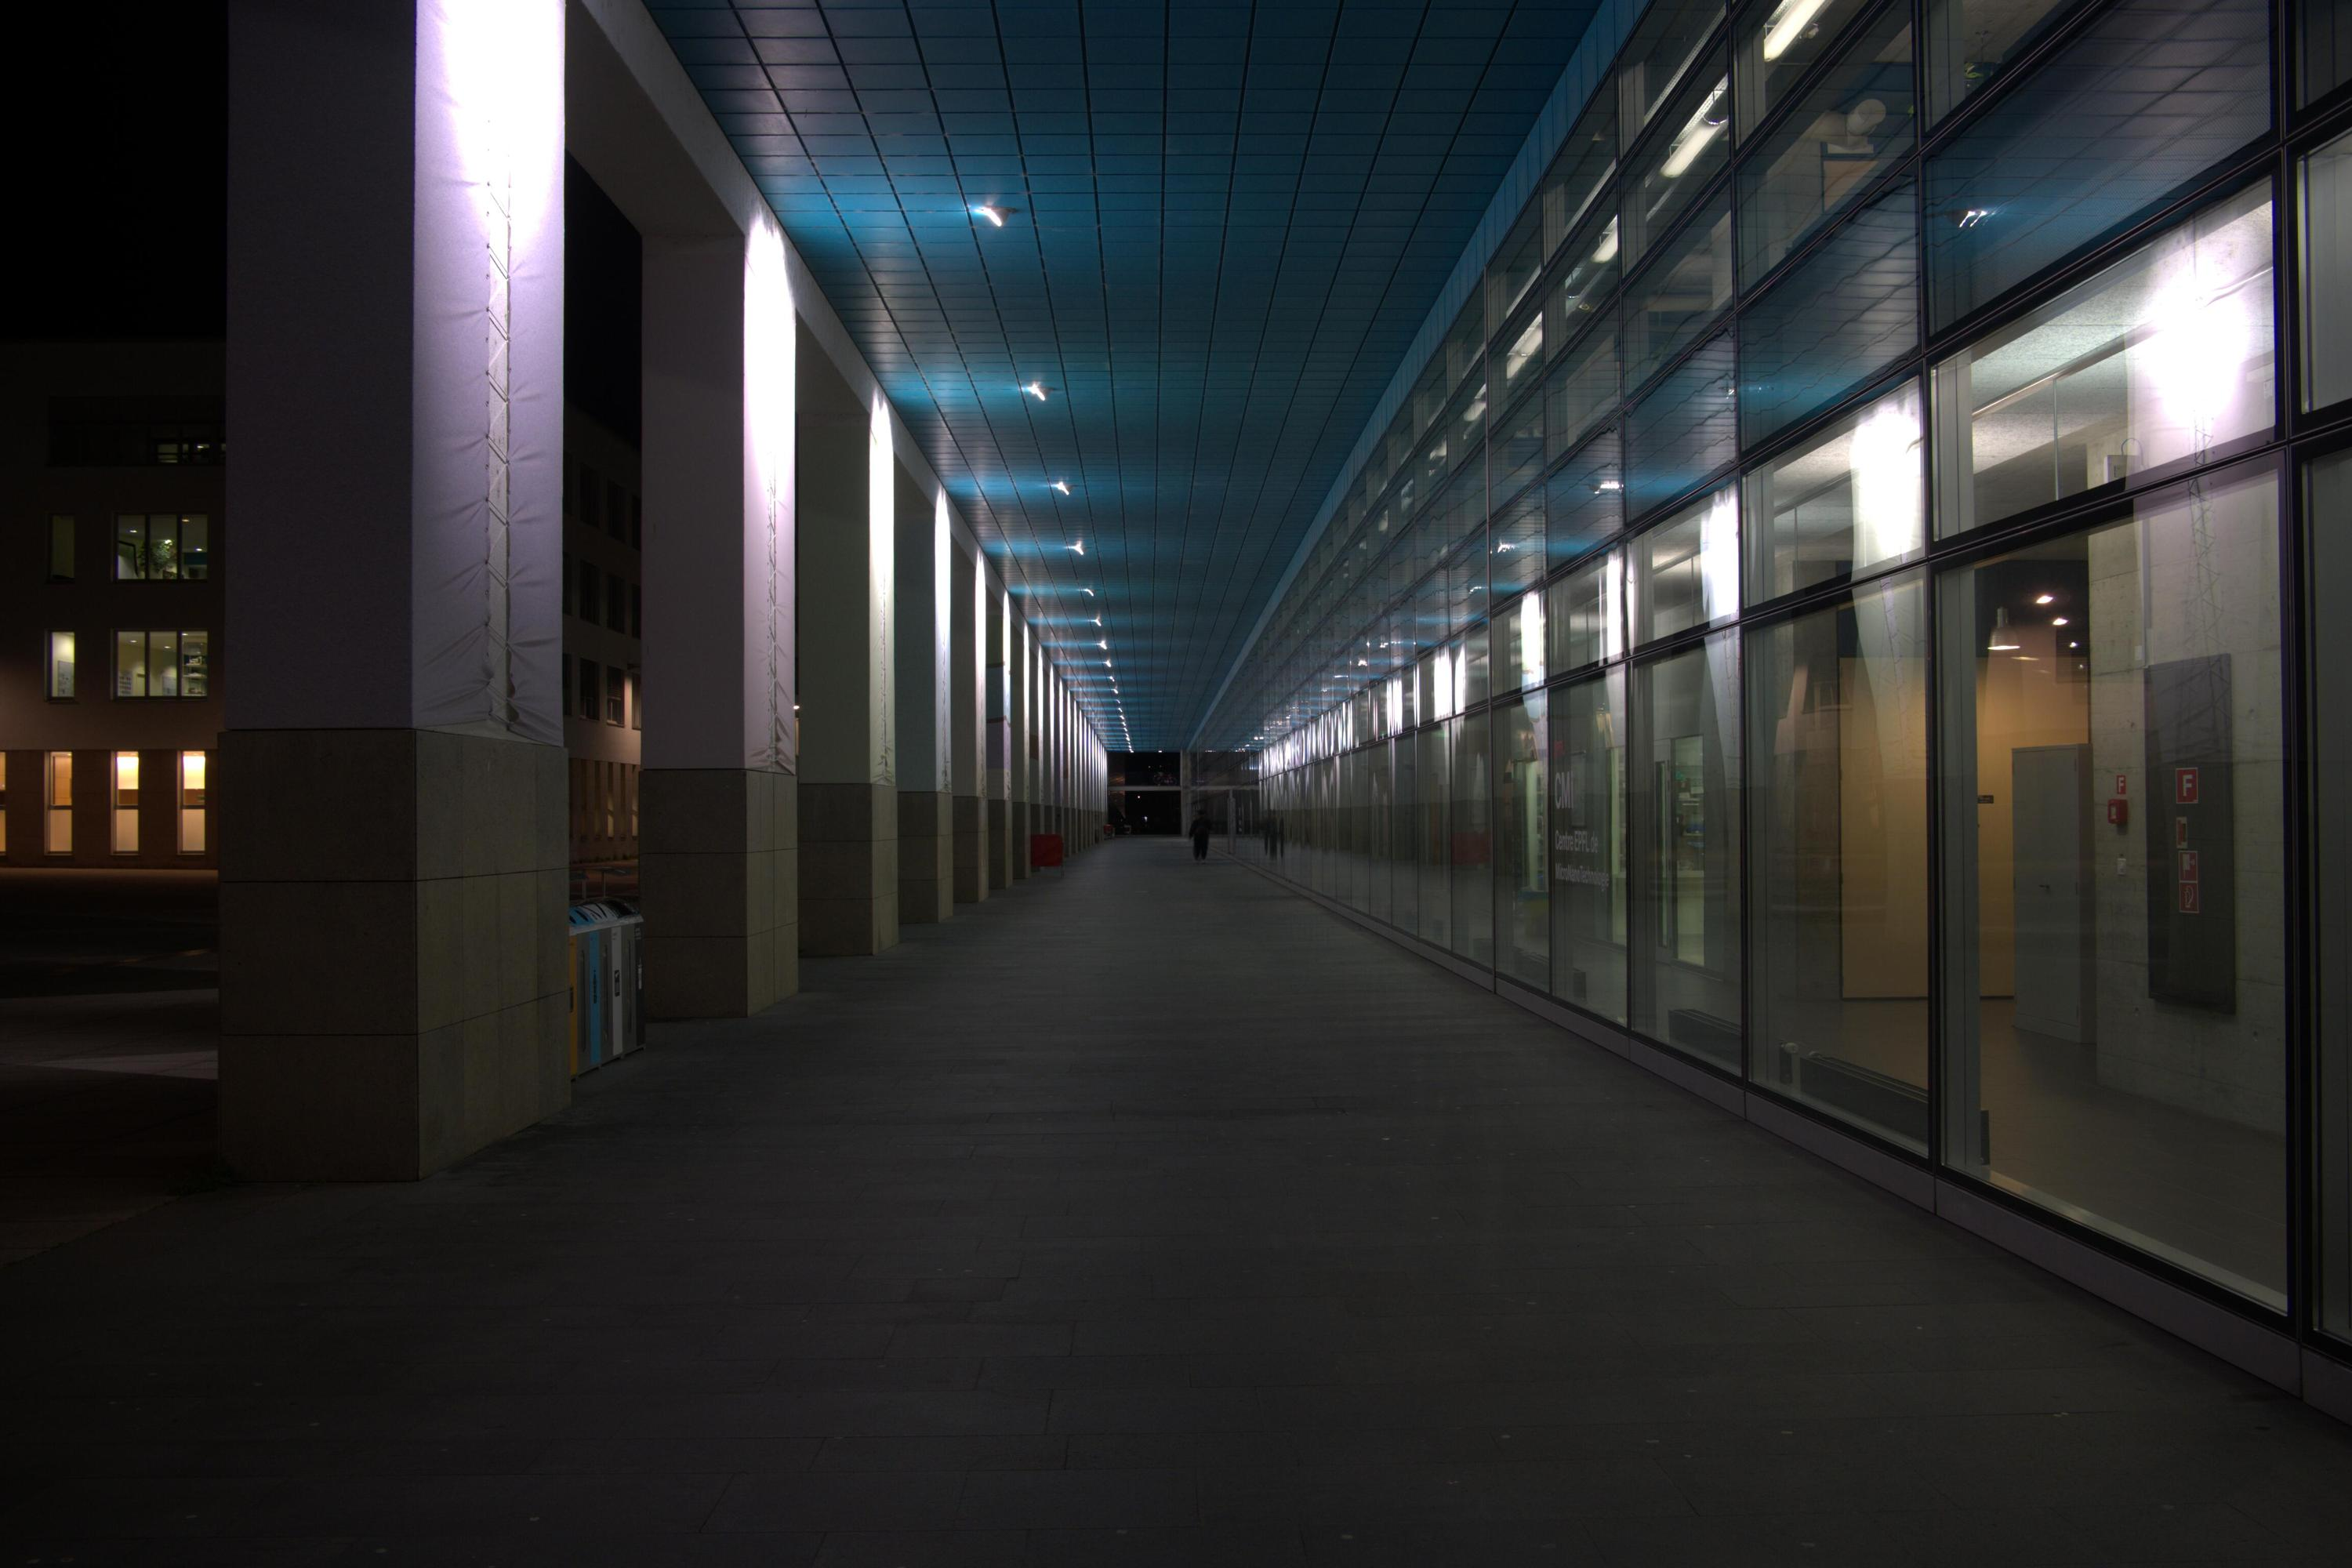
\includegraphics[width=\linewidth]{figures/digital1.jpeg}
    \end{subfigure}
    \hfill
    \begin{subfigure}[t]{.19\textwidth}
      \centering
      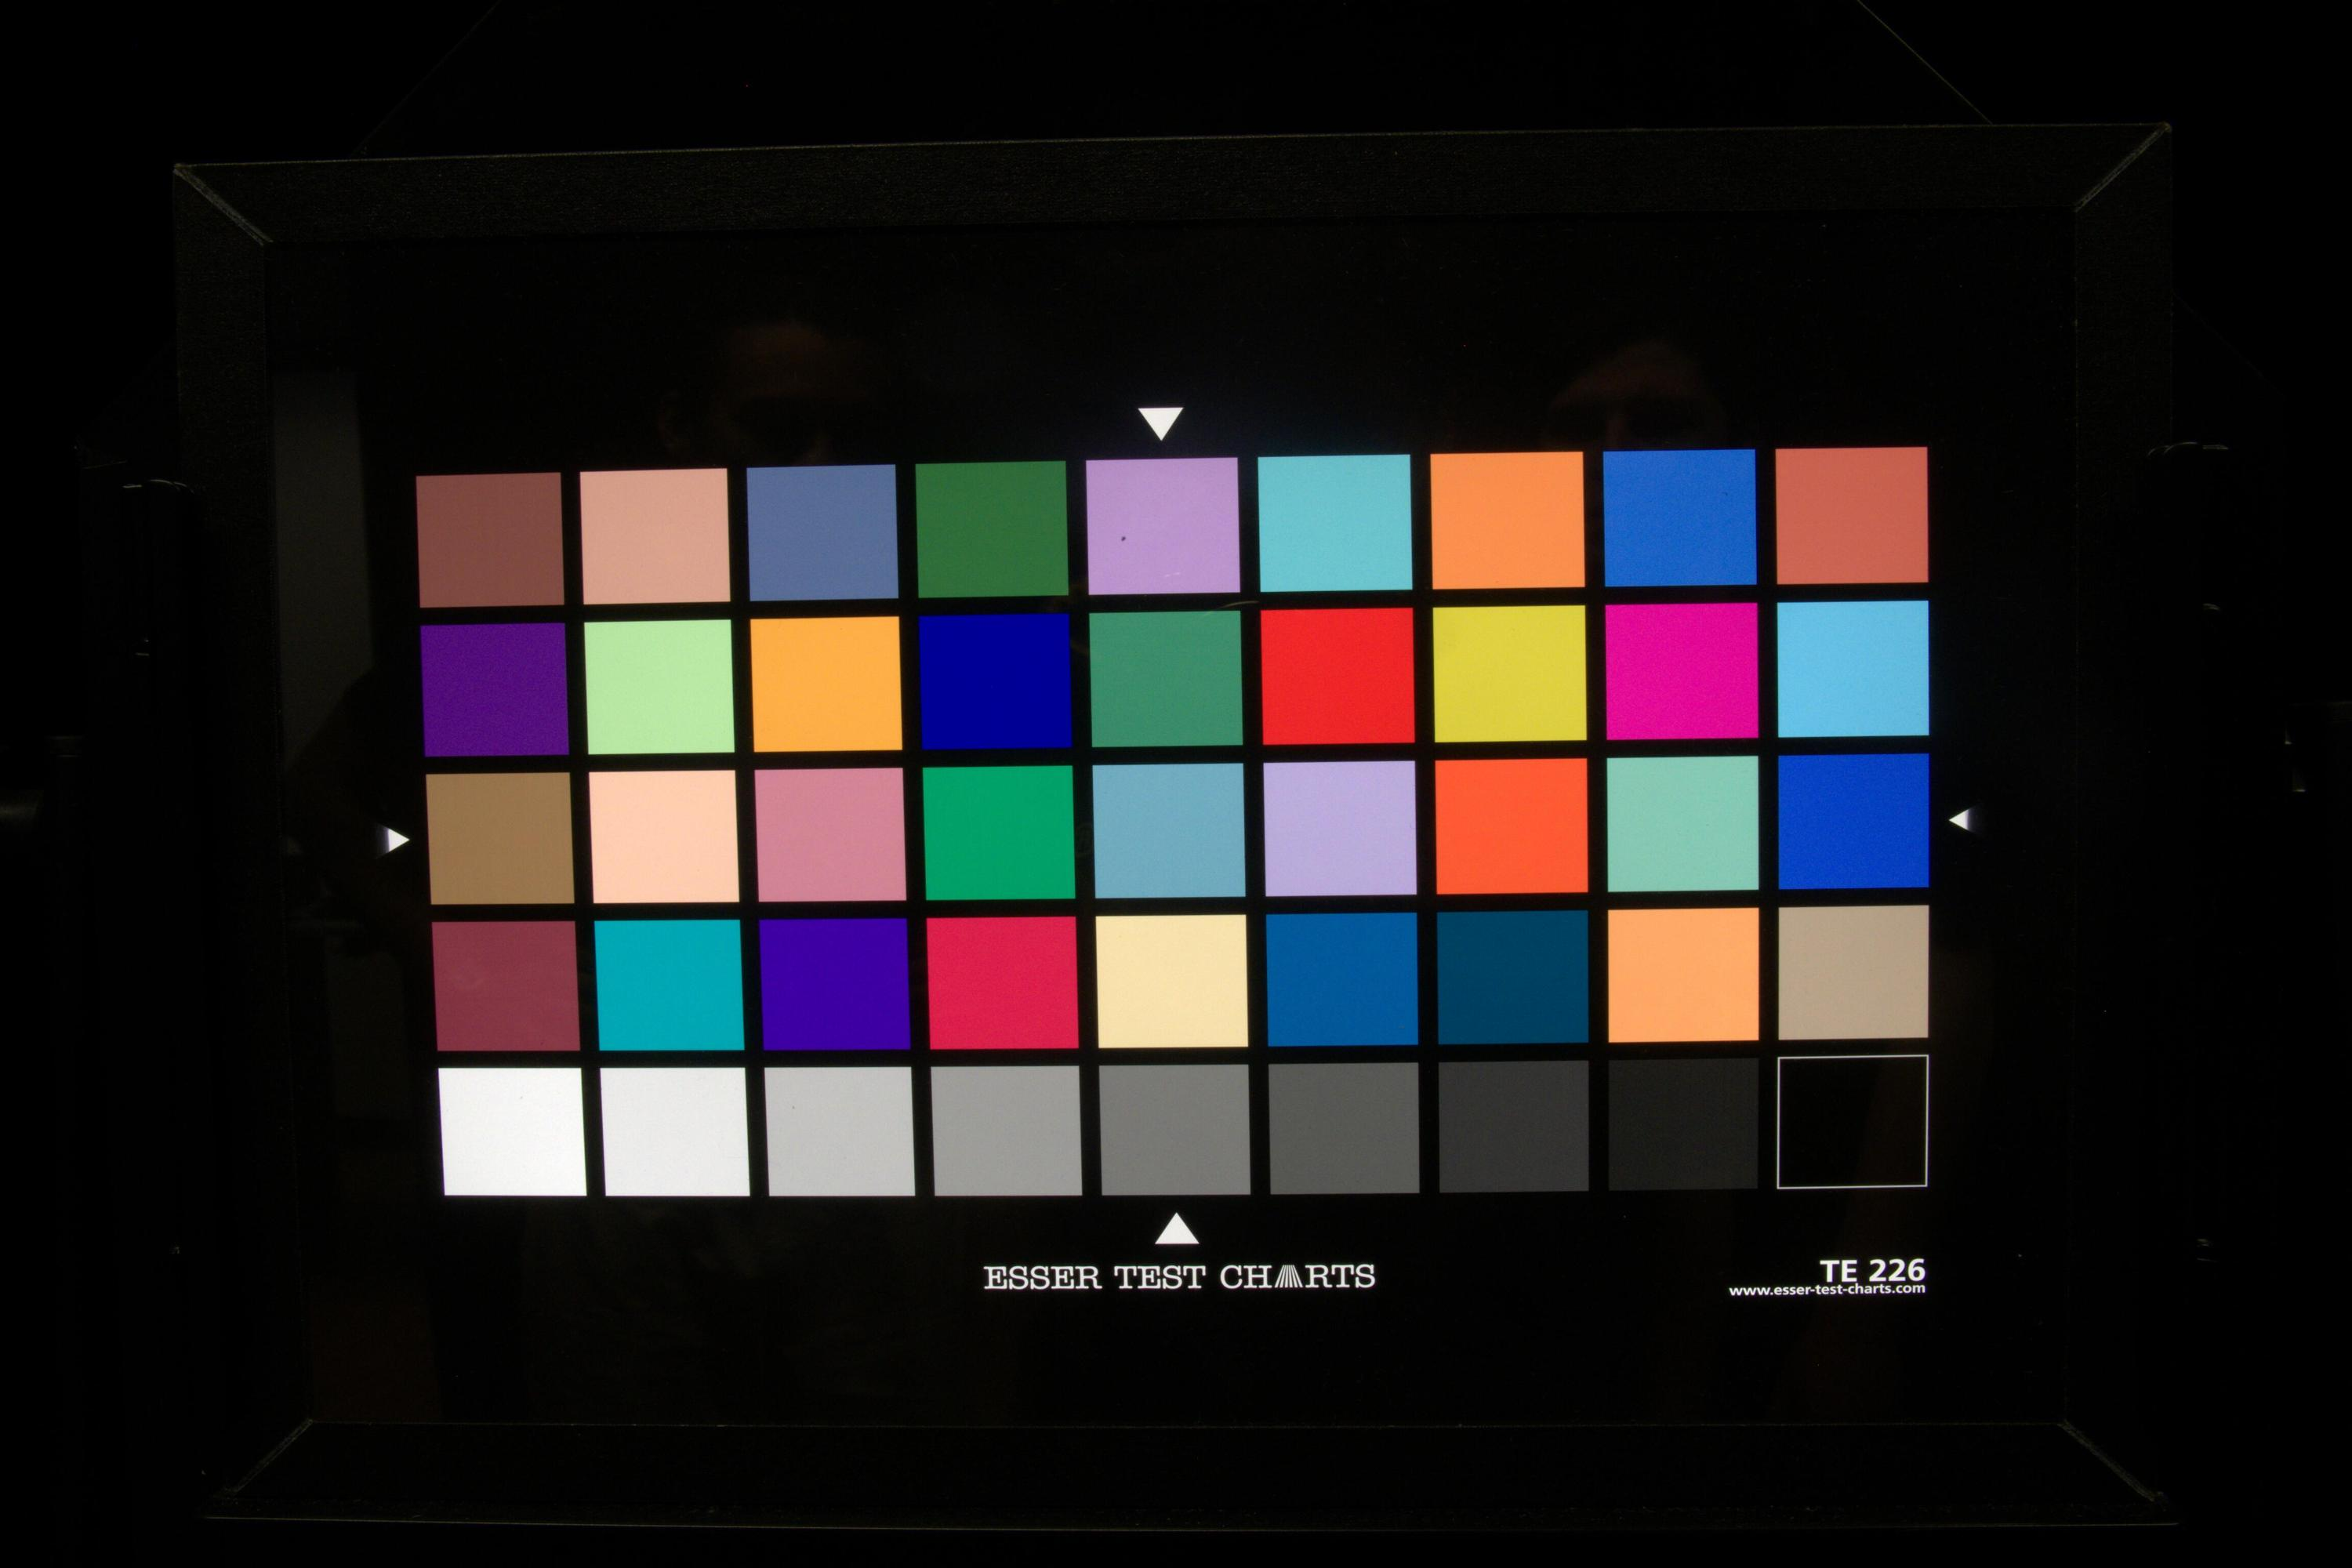
\includegraphics[width=\linewidth]{figures/digital2.jpeg}
    \end{subfigure}
    \hfill
    \begin{subfigure}[t]{.19\textwidth}
      \centering
      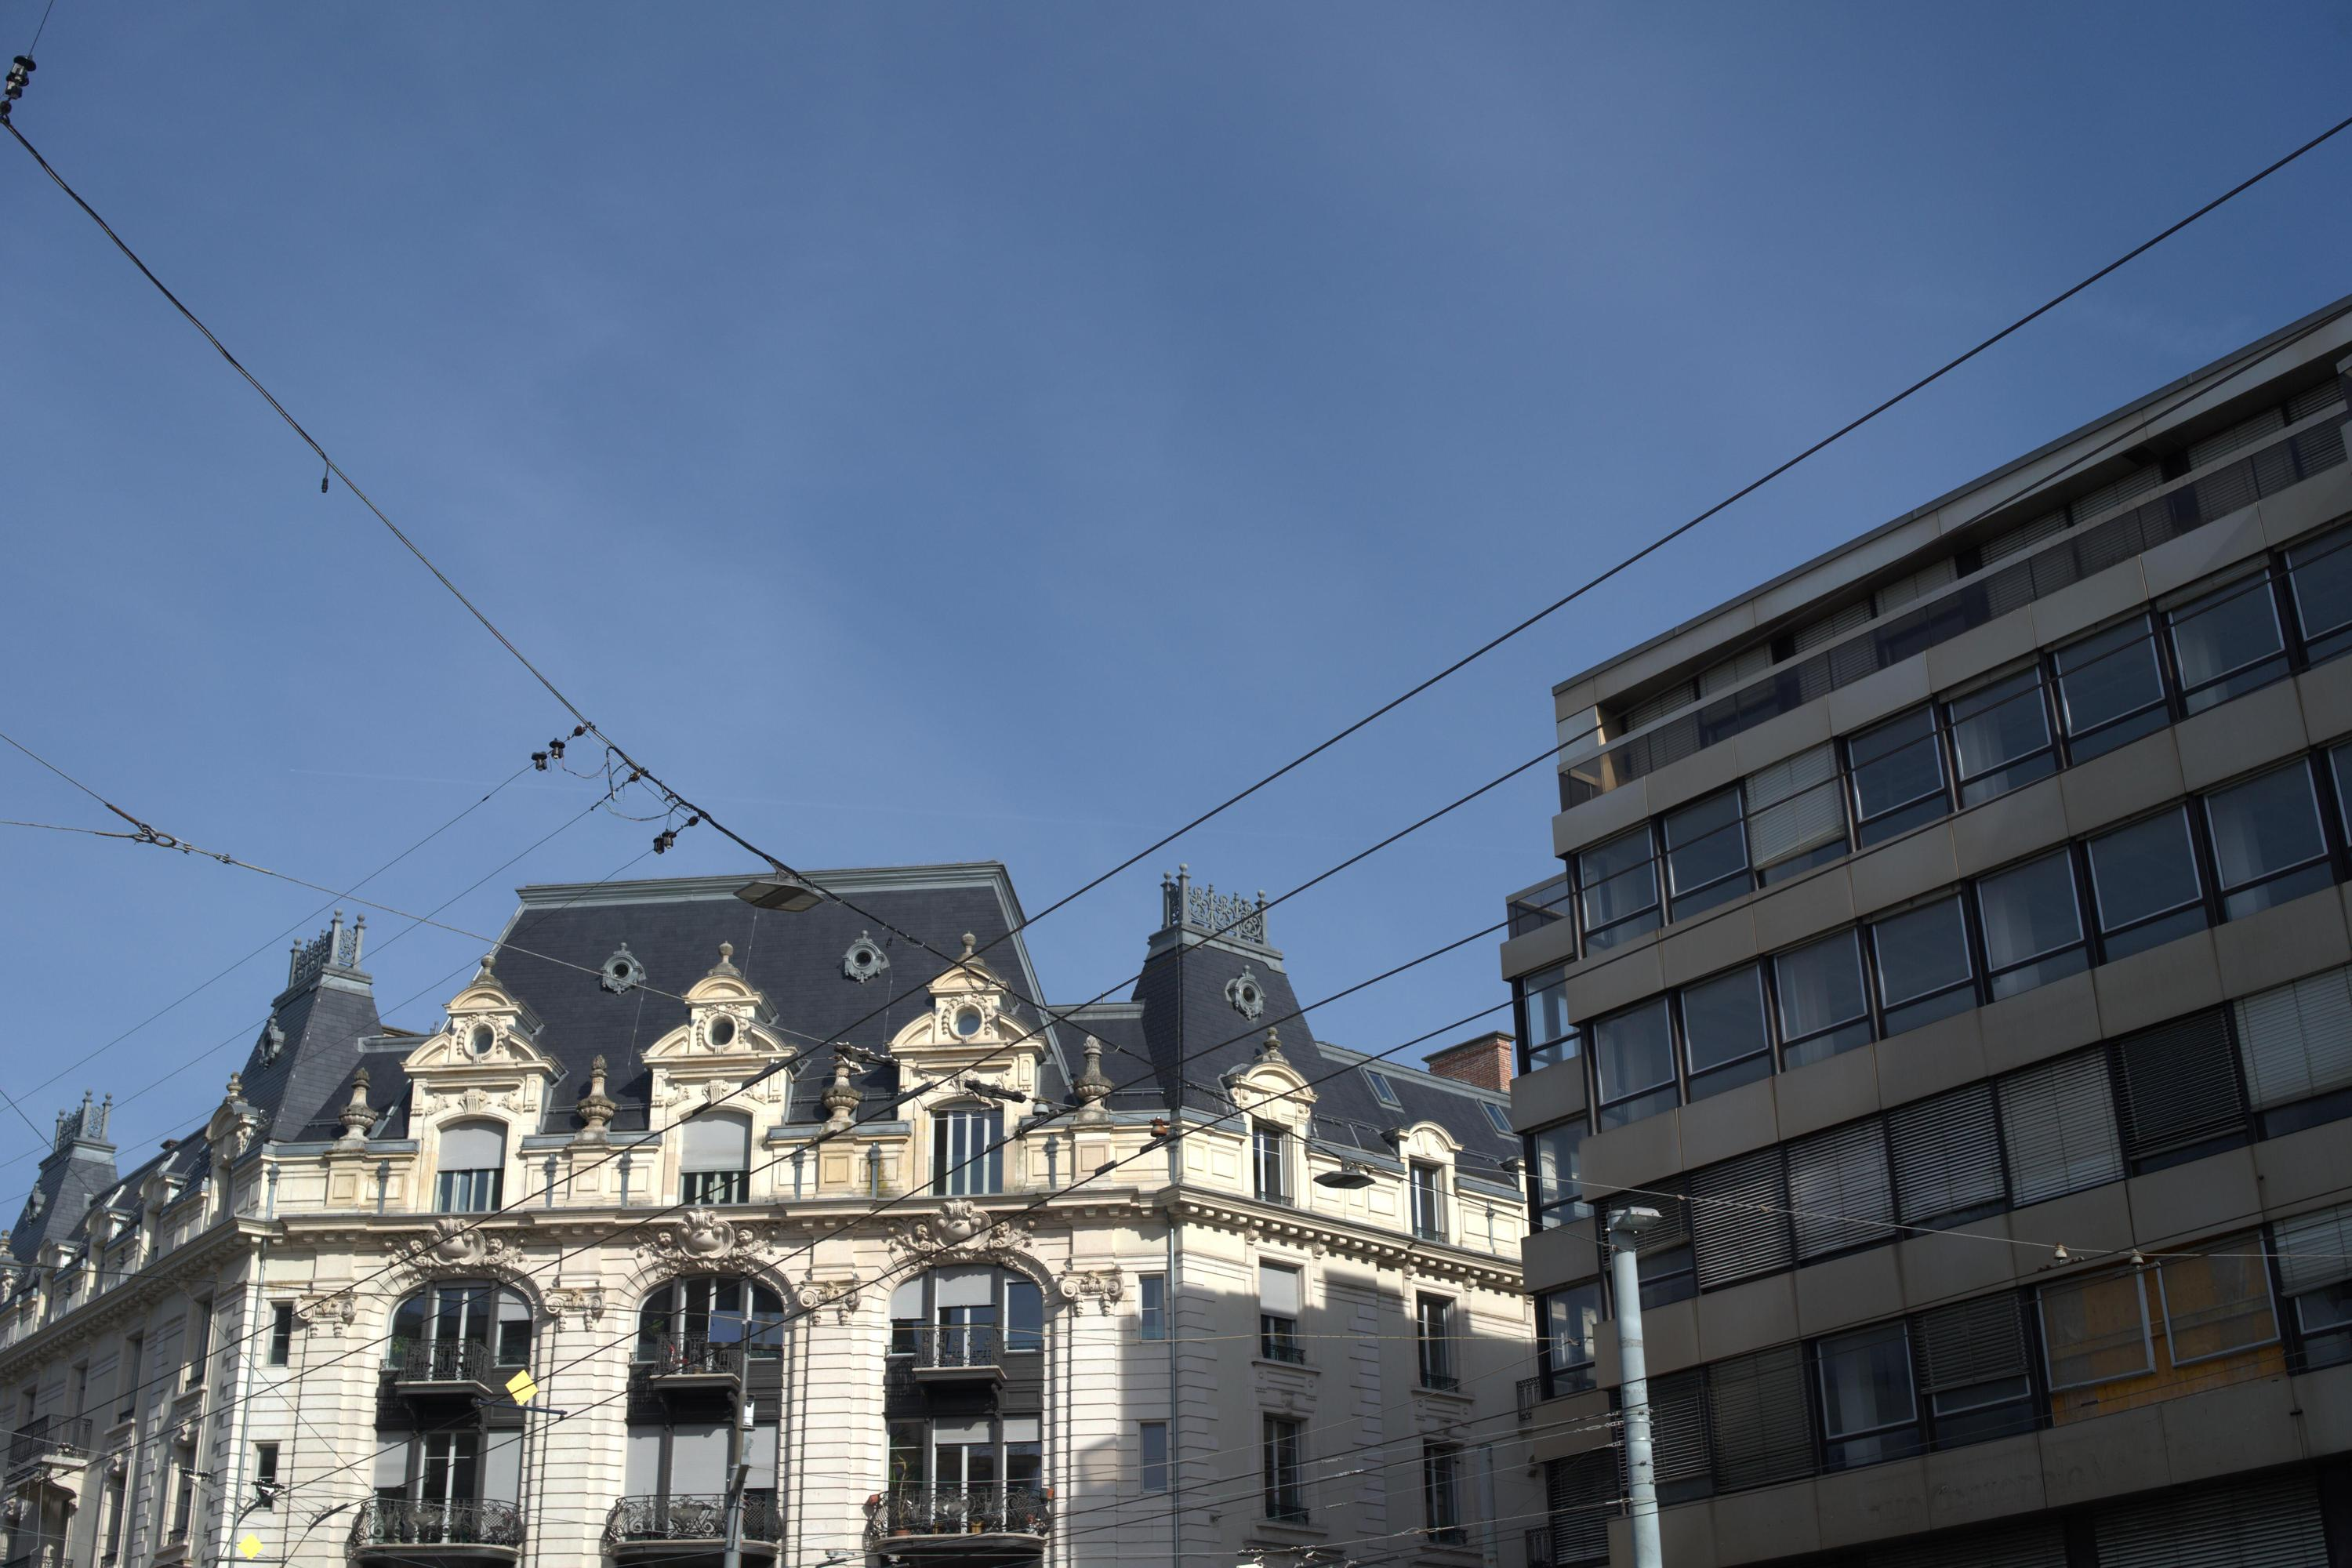
\includegraphics[width=\linewidth]{figures/digital3.jpeg}
    \end{subfigure}
    \hfill
    \begin{subfigure}[t]{.19\textwidth}
      \centering
      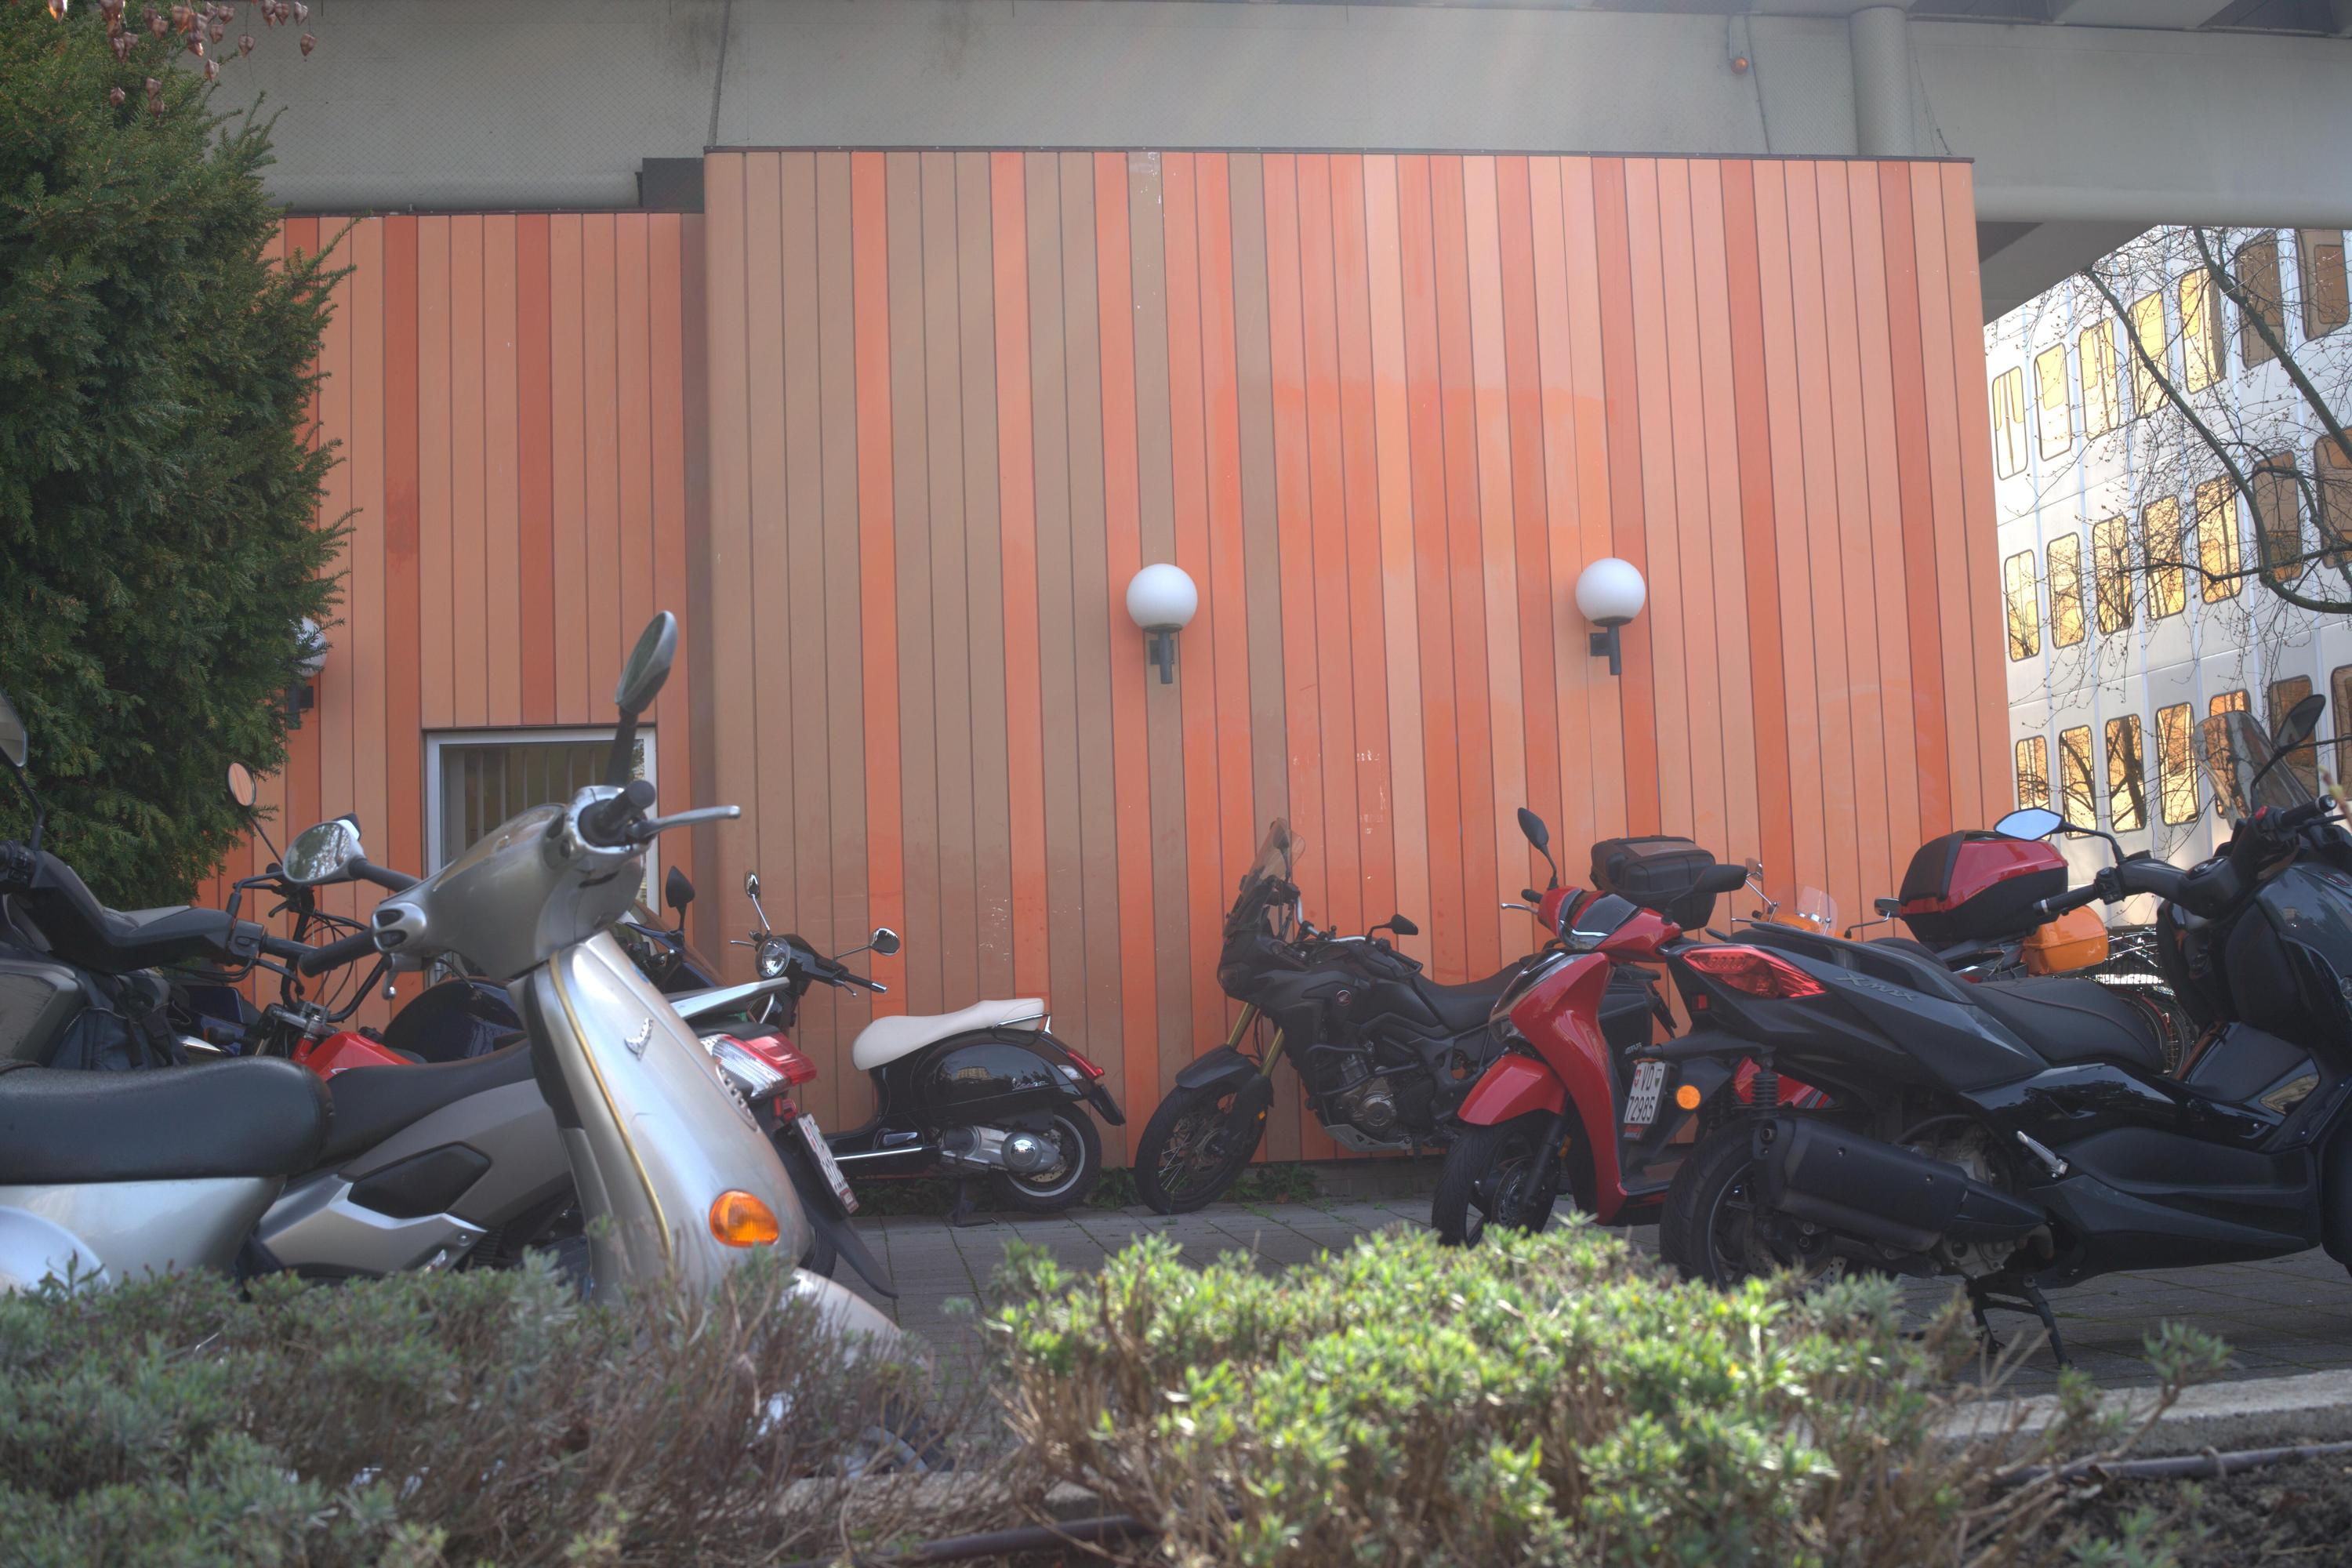
\includegraphics[width=\linewidth]{figures/digital4.jpeg}
    \end{subfigure}
    \begin{subfigure}[t]{.19\textwidth}
      \centering
      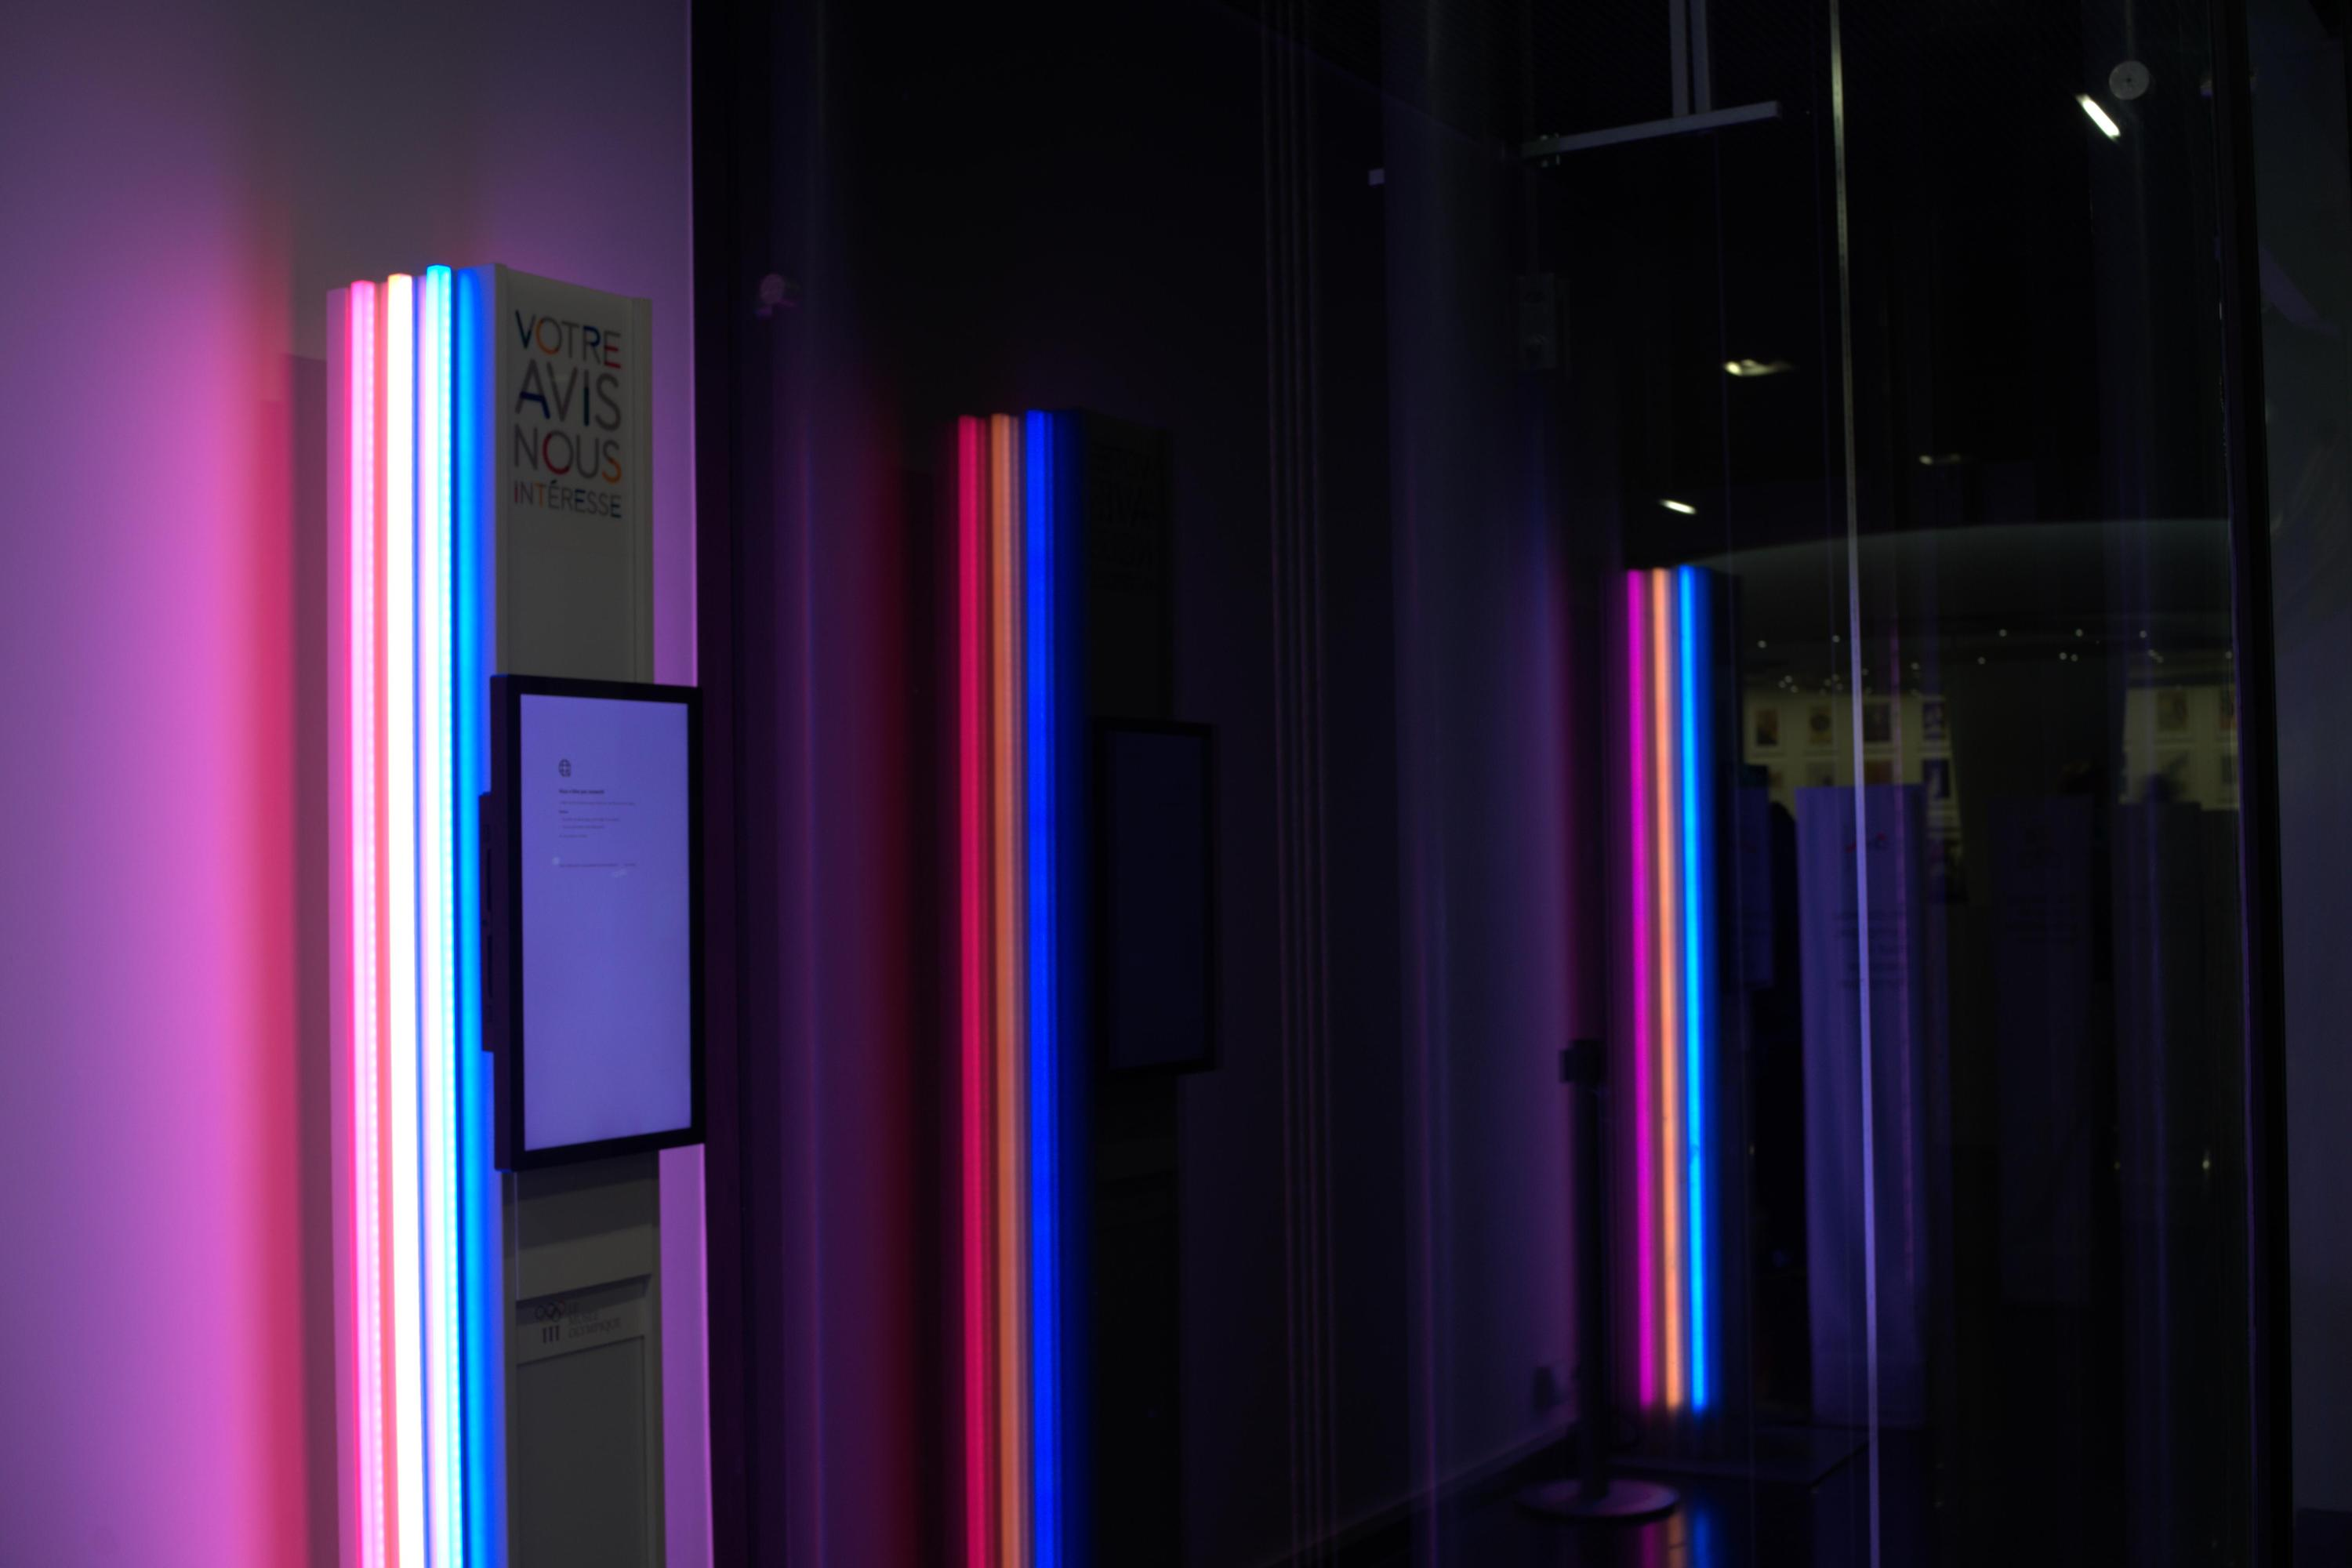
\includegraphics[width=\linewidth]{figures/digital5.jpeg}
    \end{subfigure}
  
    \medskip

    \begin{subfigure}[t]{.19\textwidth}
      \centering
      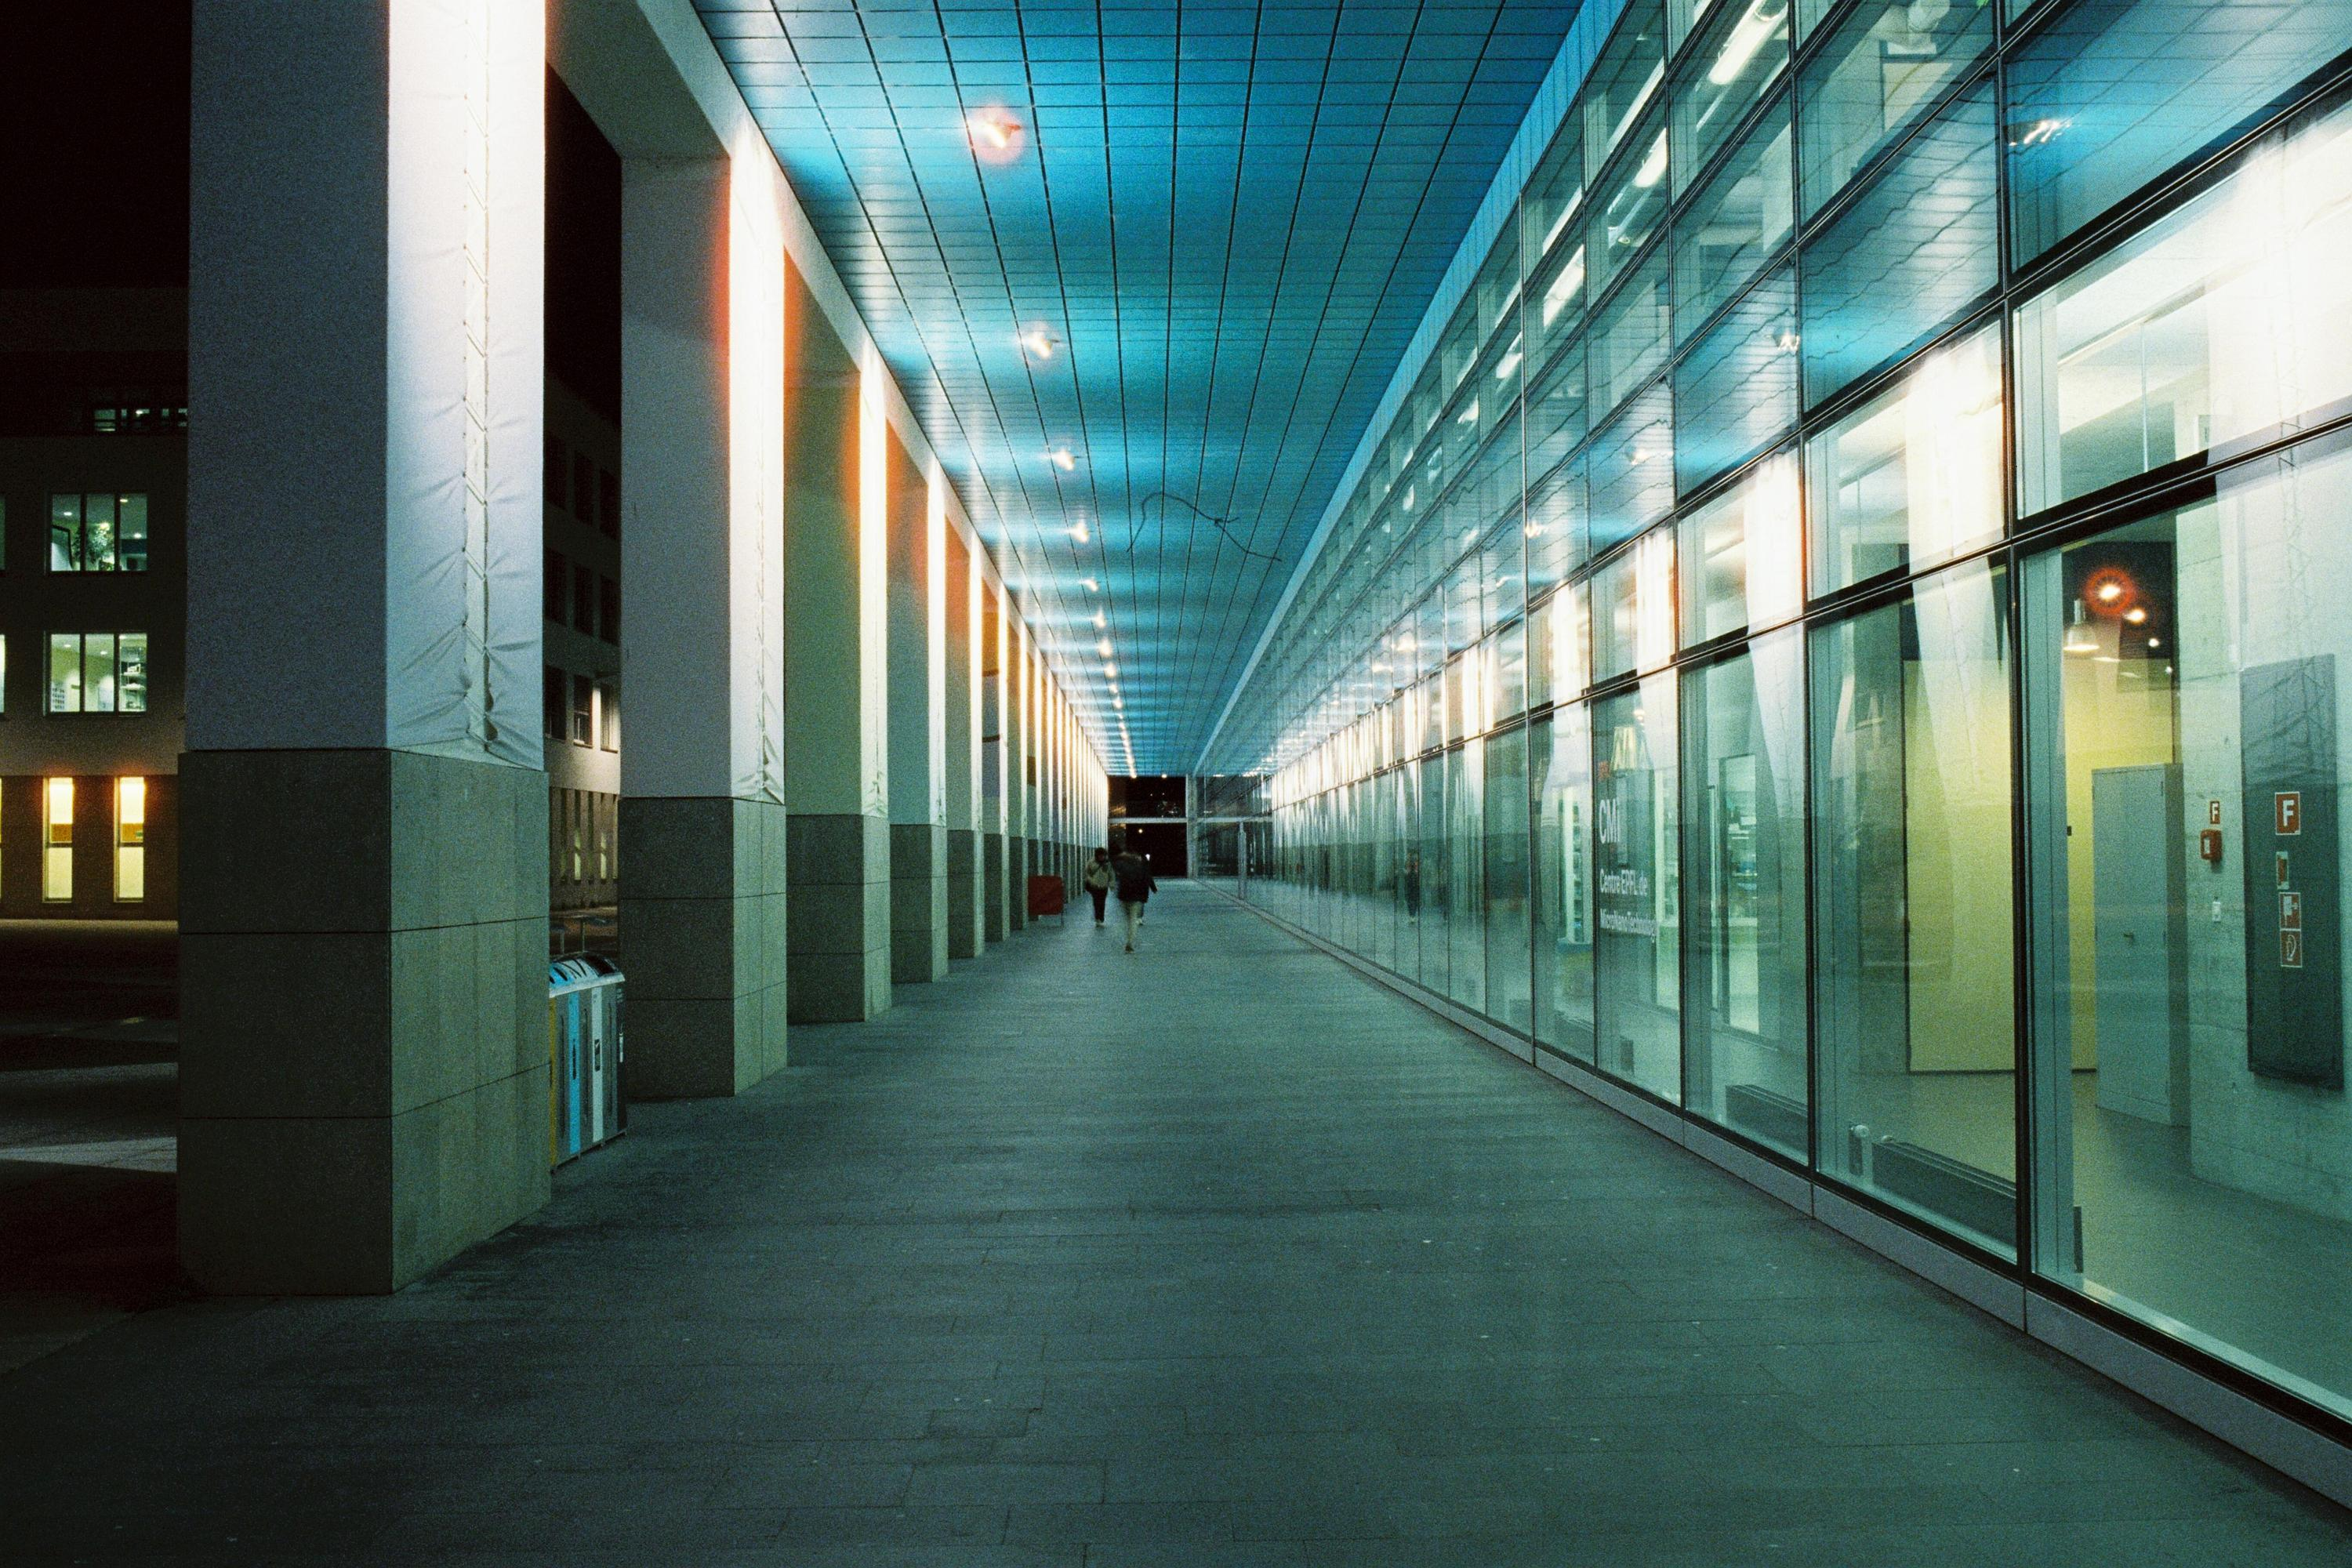
\includegraphics[width=\linewidth]{figures/film1.jpeg}
      \caption{Pair 1}
    \end{subfigure}
    \hfill
    \begin{subfigure}[t]{.19\textwidth}
      \centering
      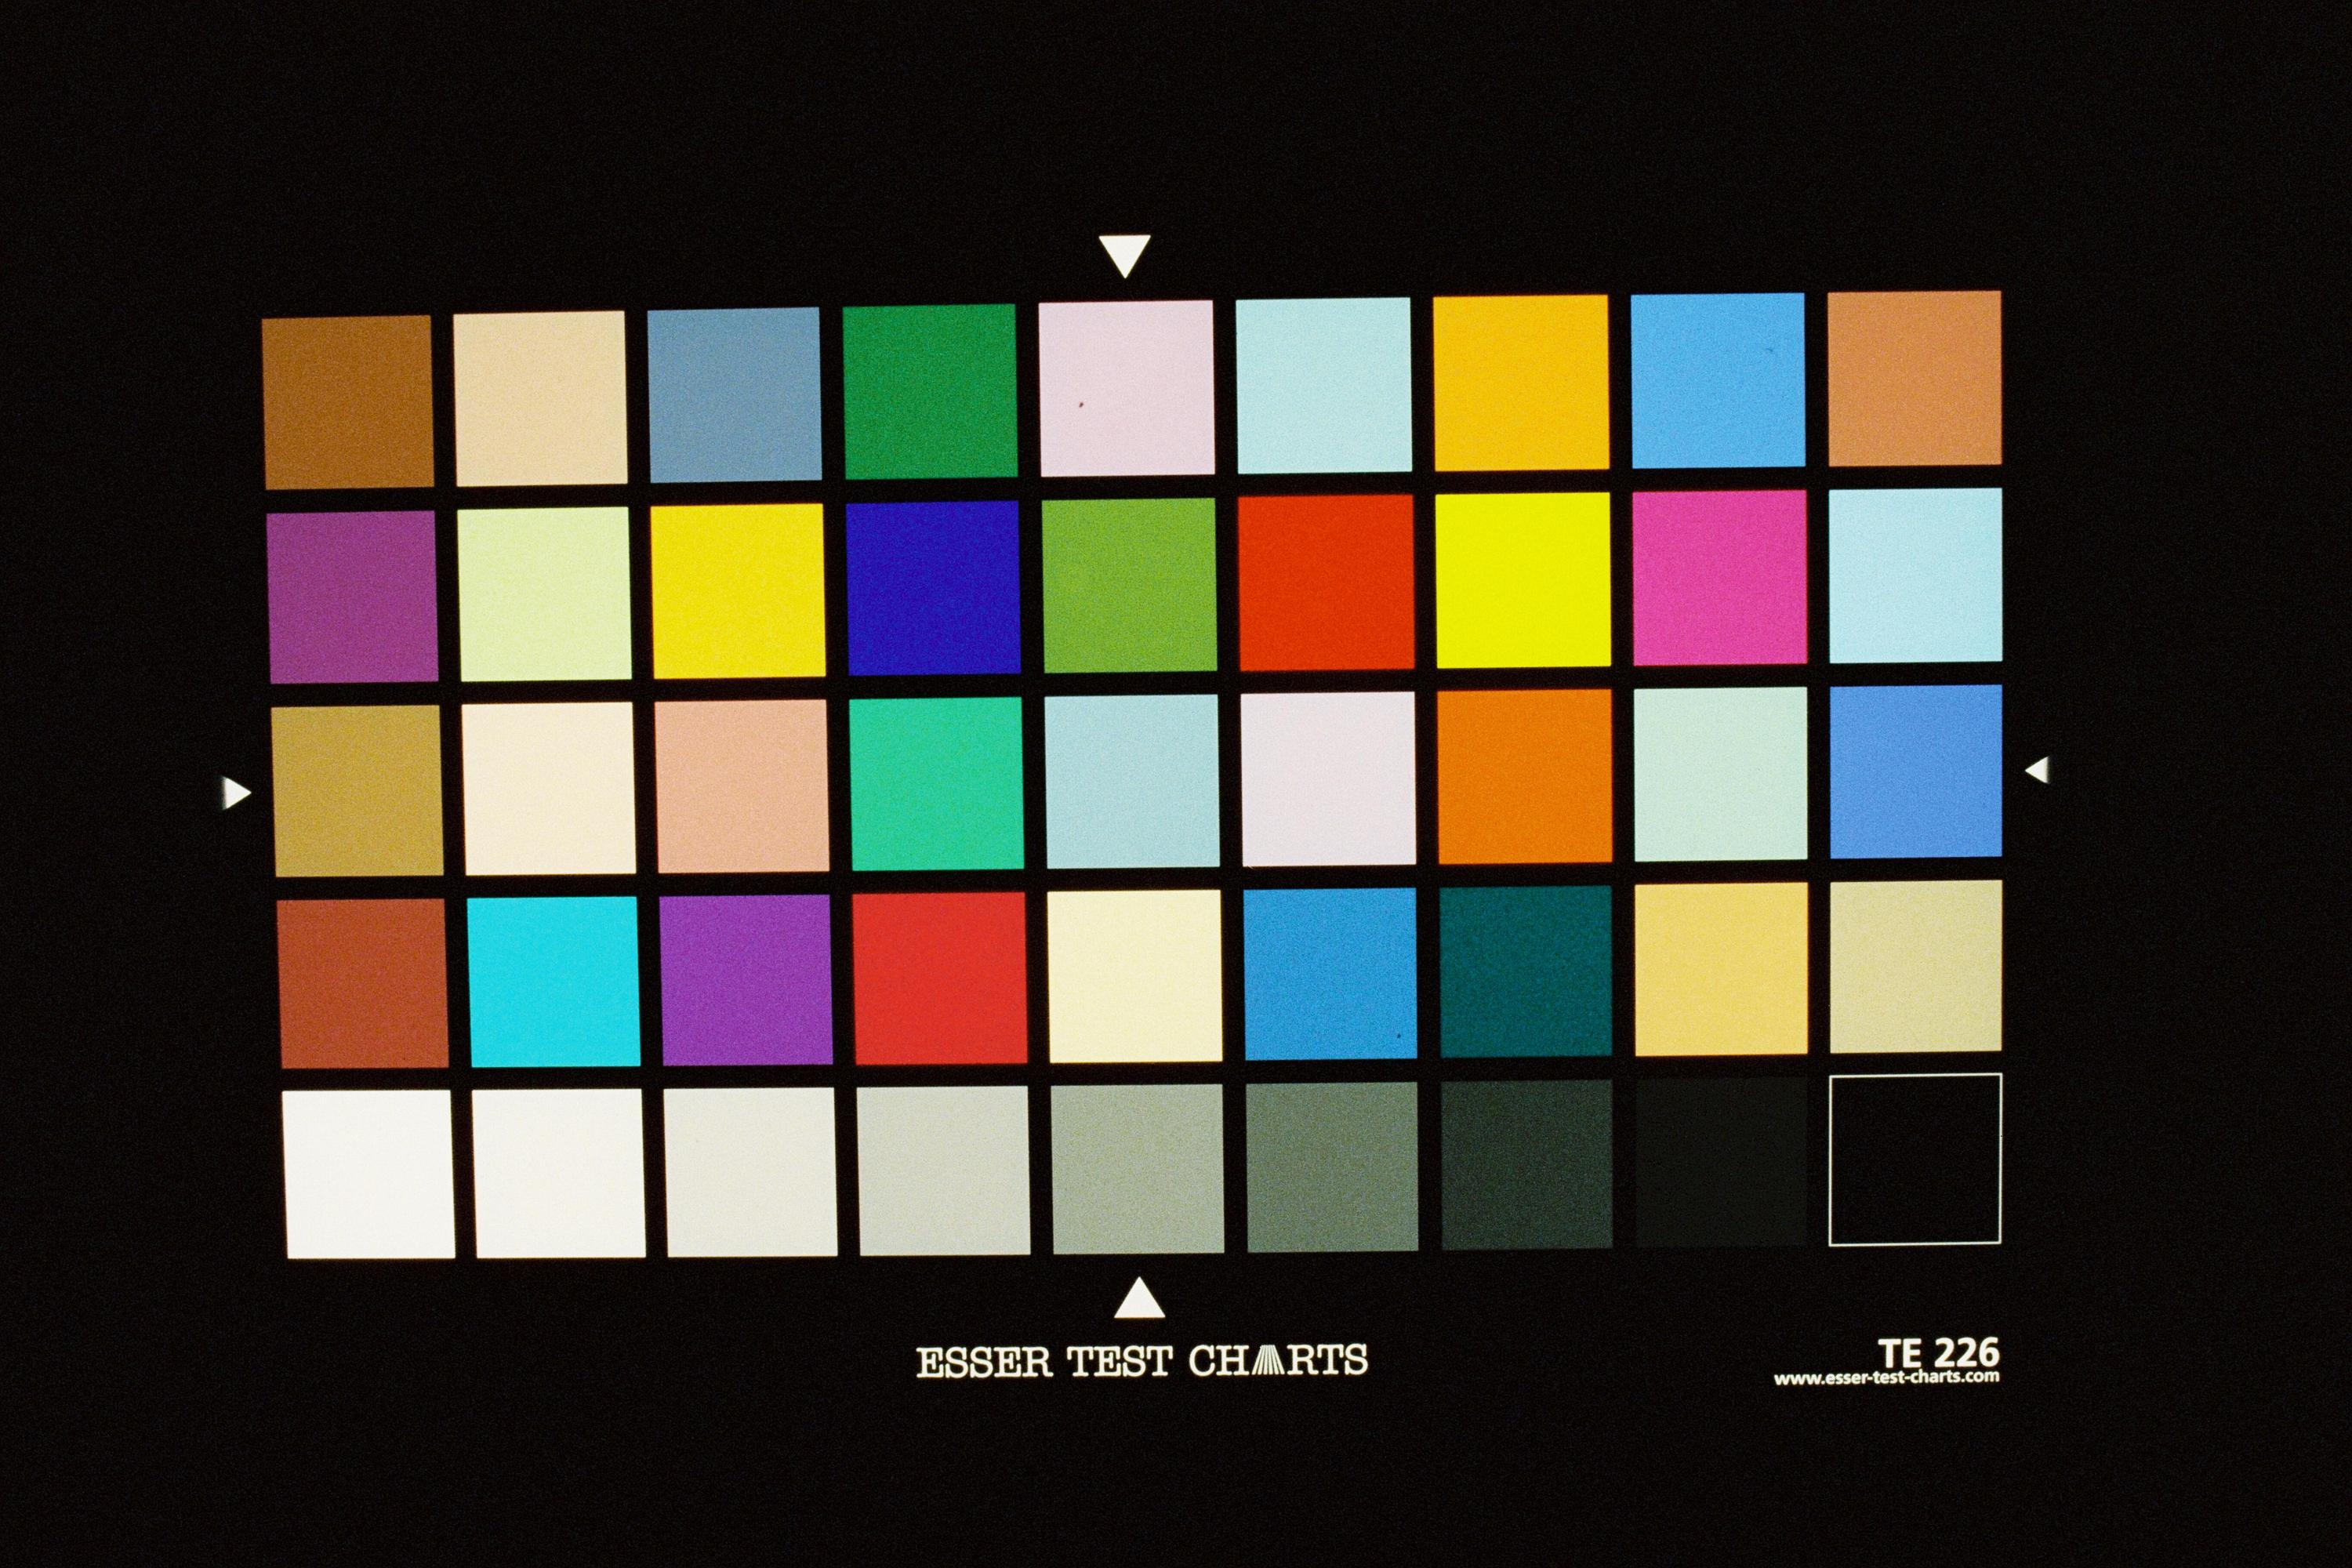
\includegraphics[width=\linewidth]{figures/film2.jpeg}
      \caption{Pair 2}
    \end{subfigure}
    \hfill
    \begin{subfigure}[t]{.19\textwidth}
      \centering
      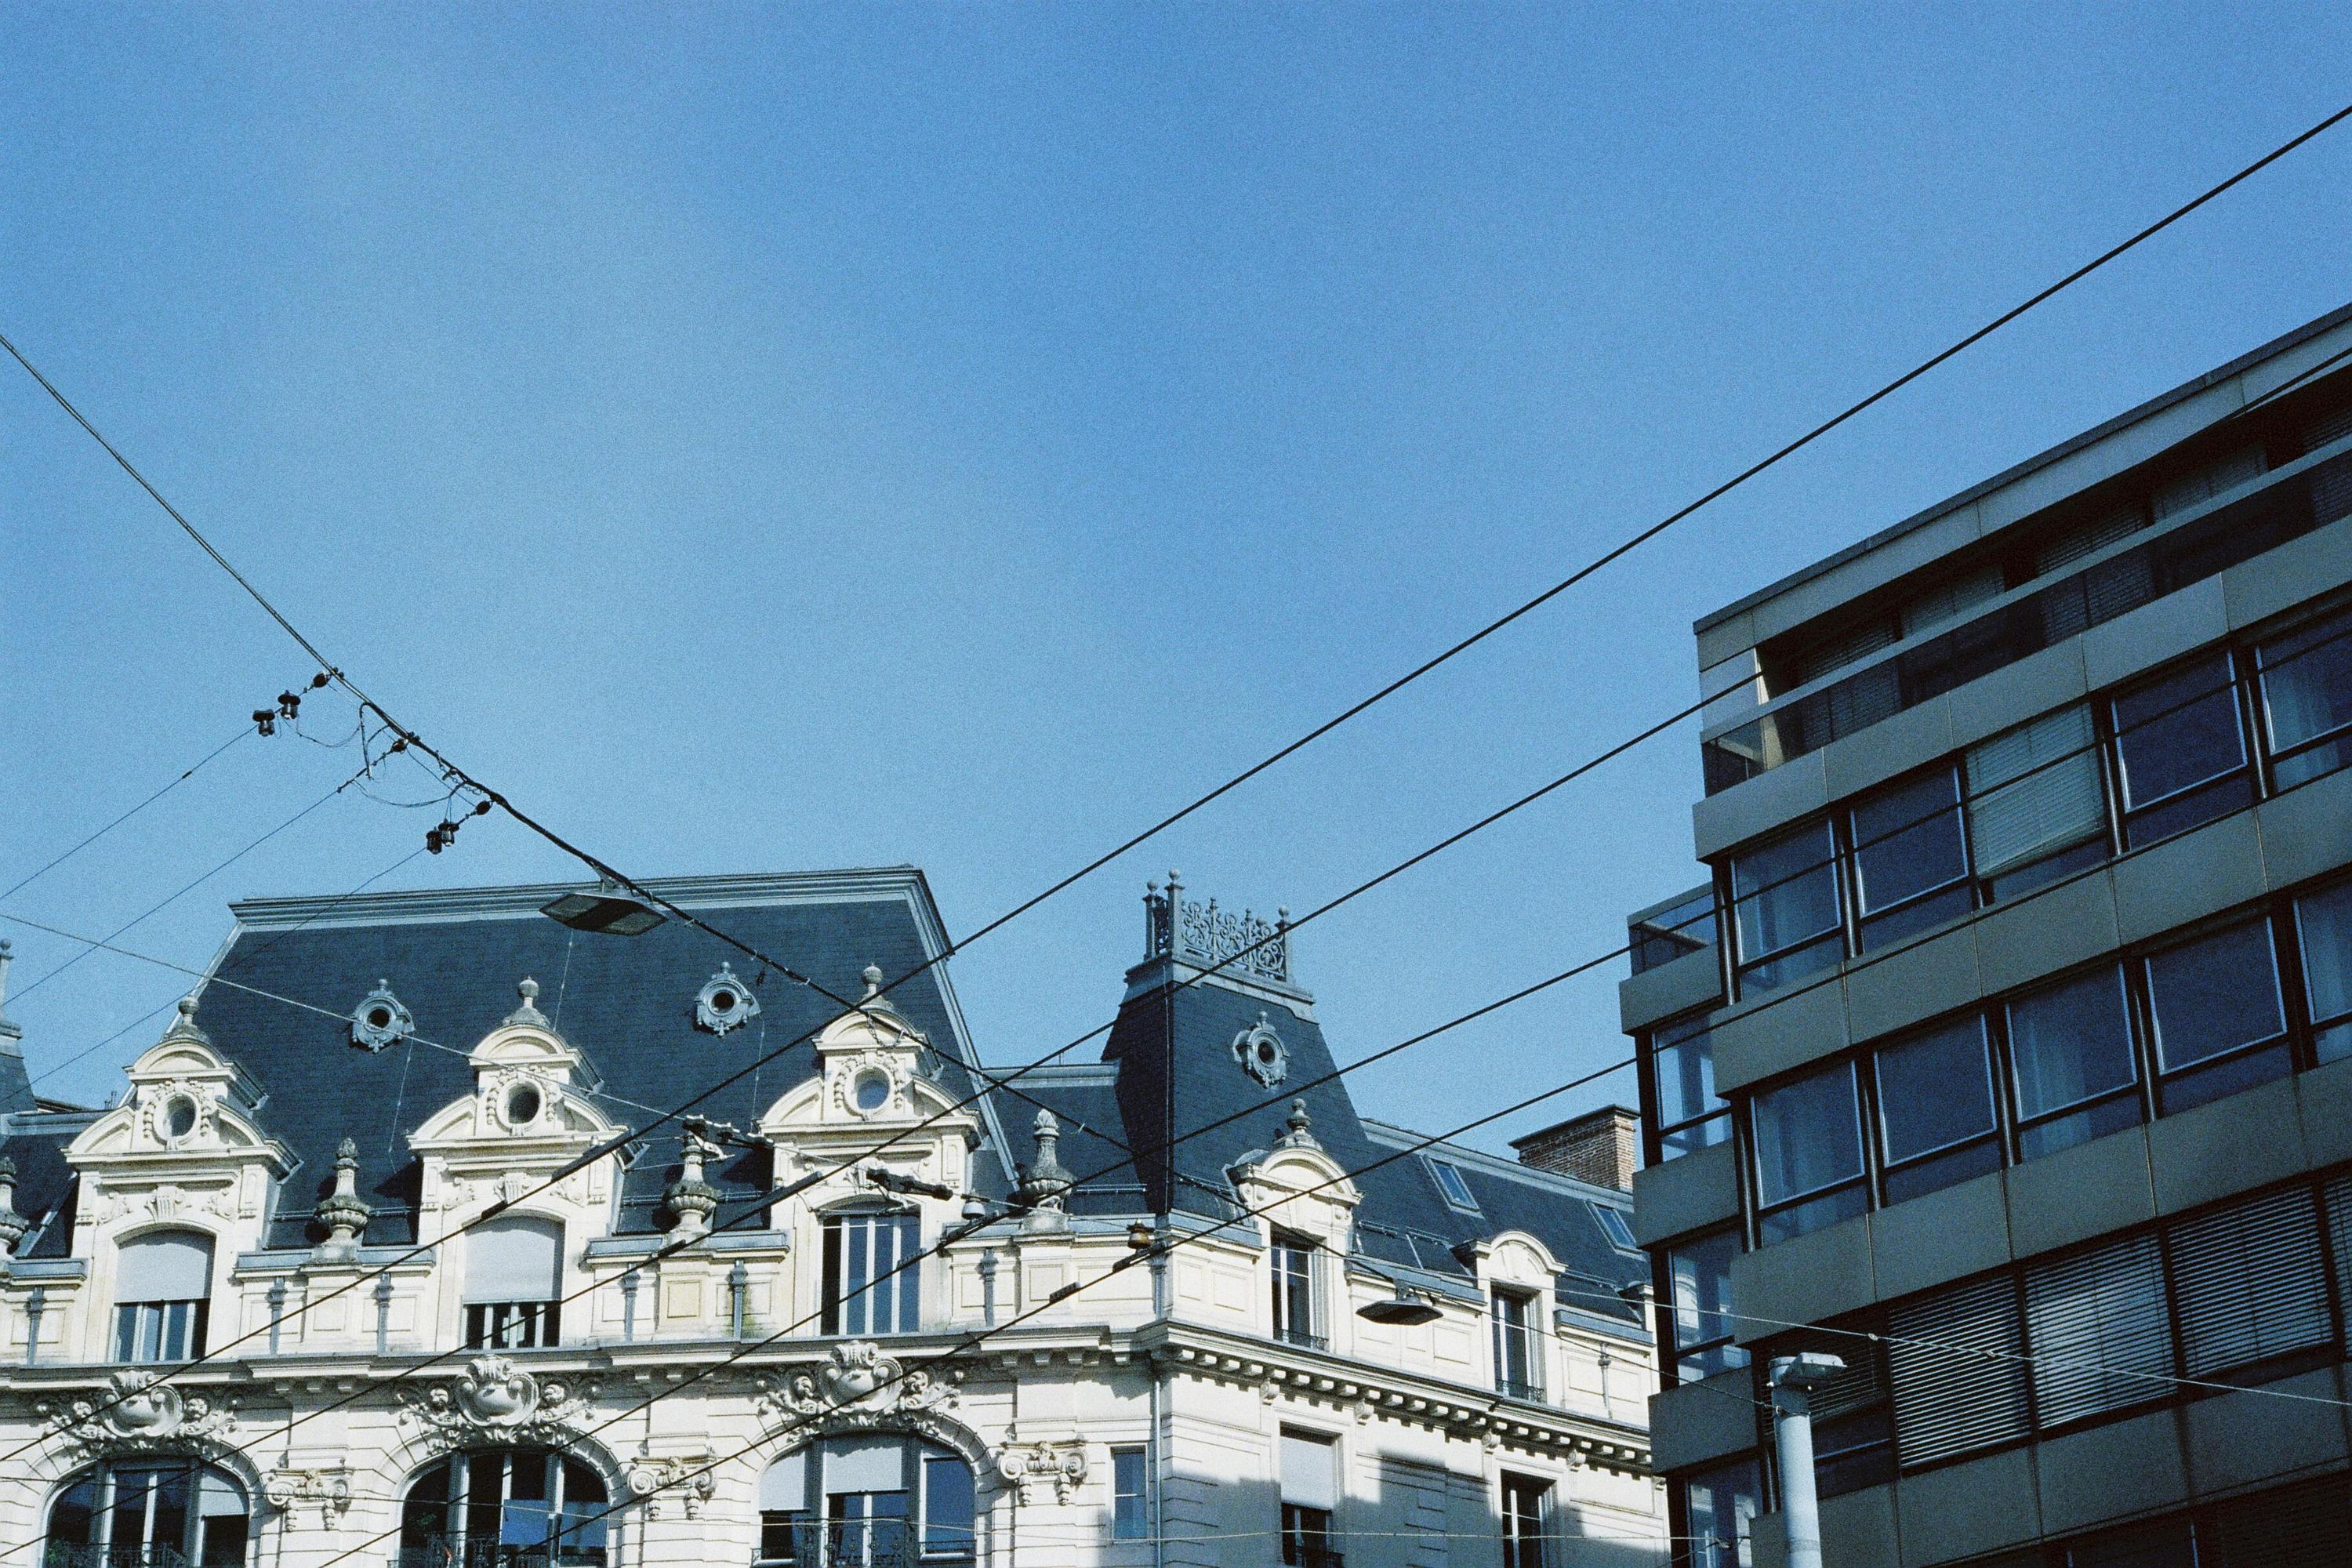
\includegraphics[width=\linewidth]{figures/film3.jpeg}
      \caption{Pair 3}
    \end{subfigure}
    \hfill
    \begin{subfigure}[t]{.19\textwidth}
      \centering
      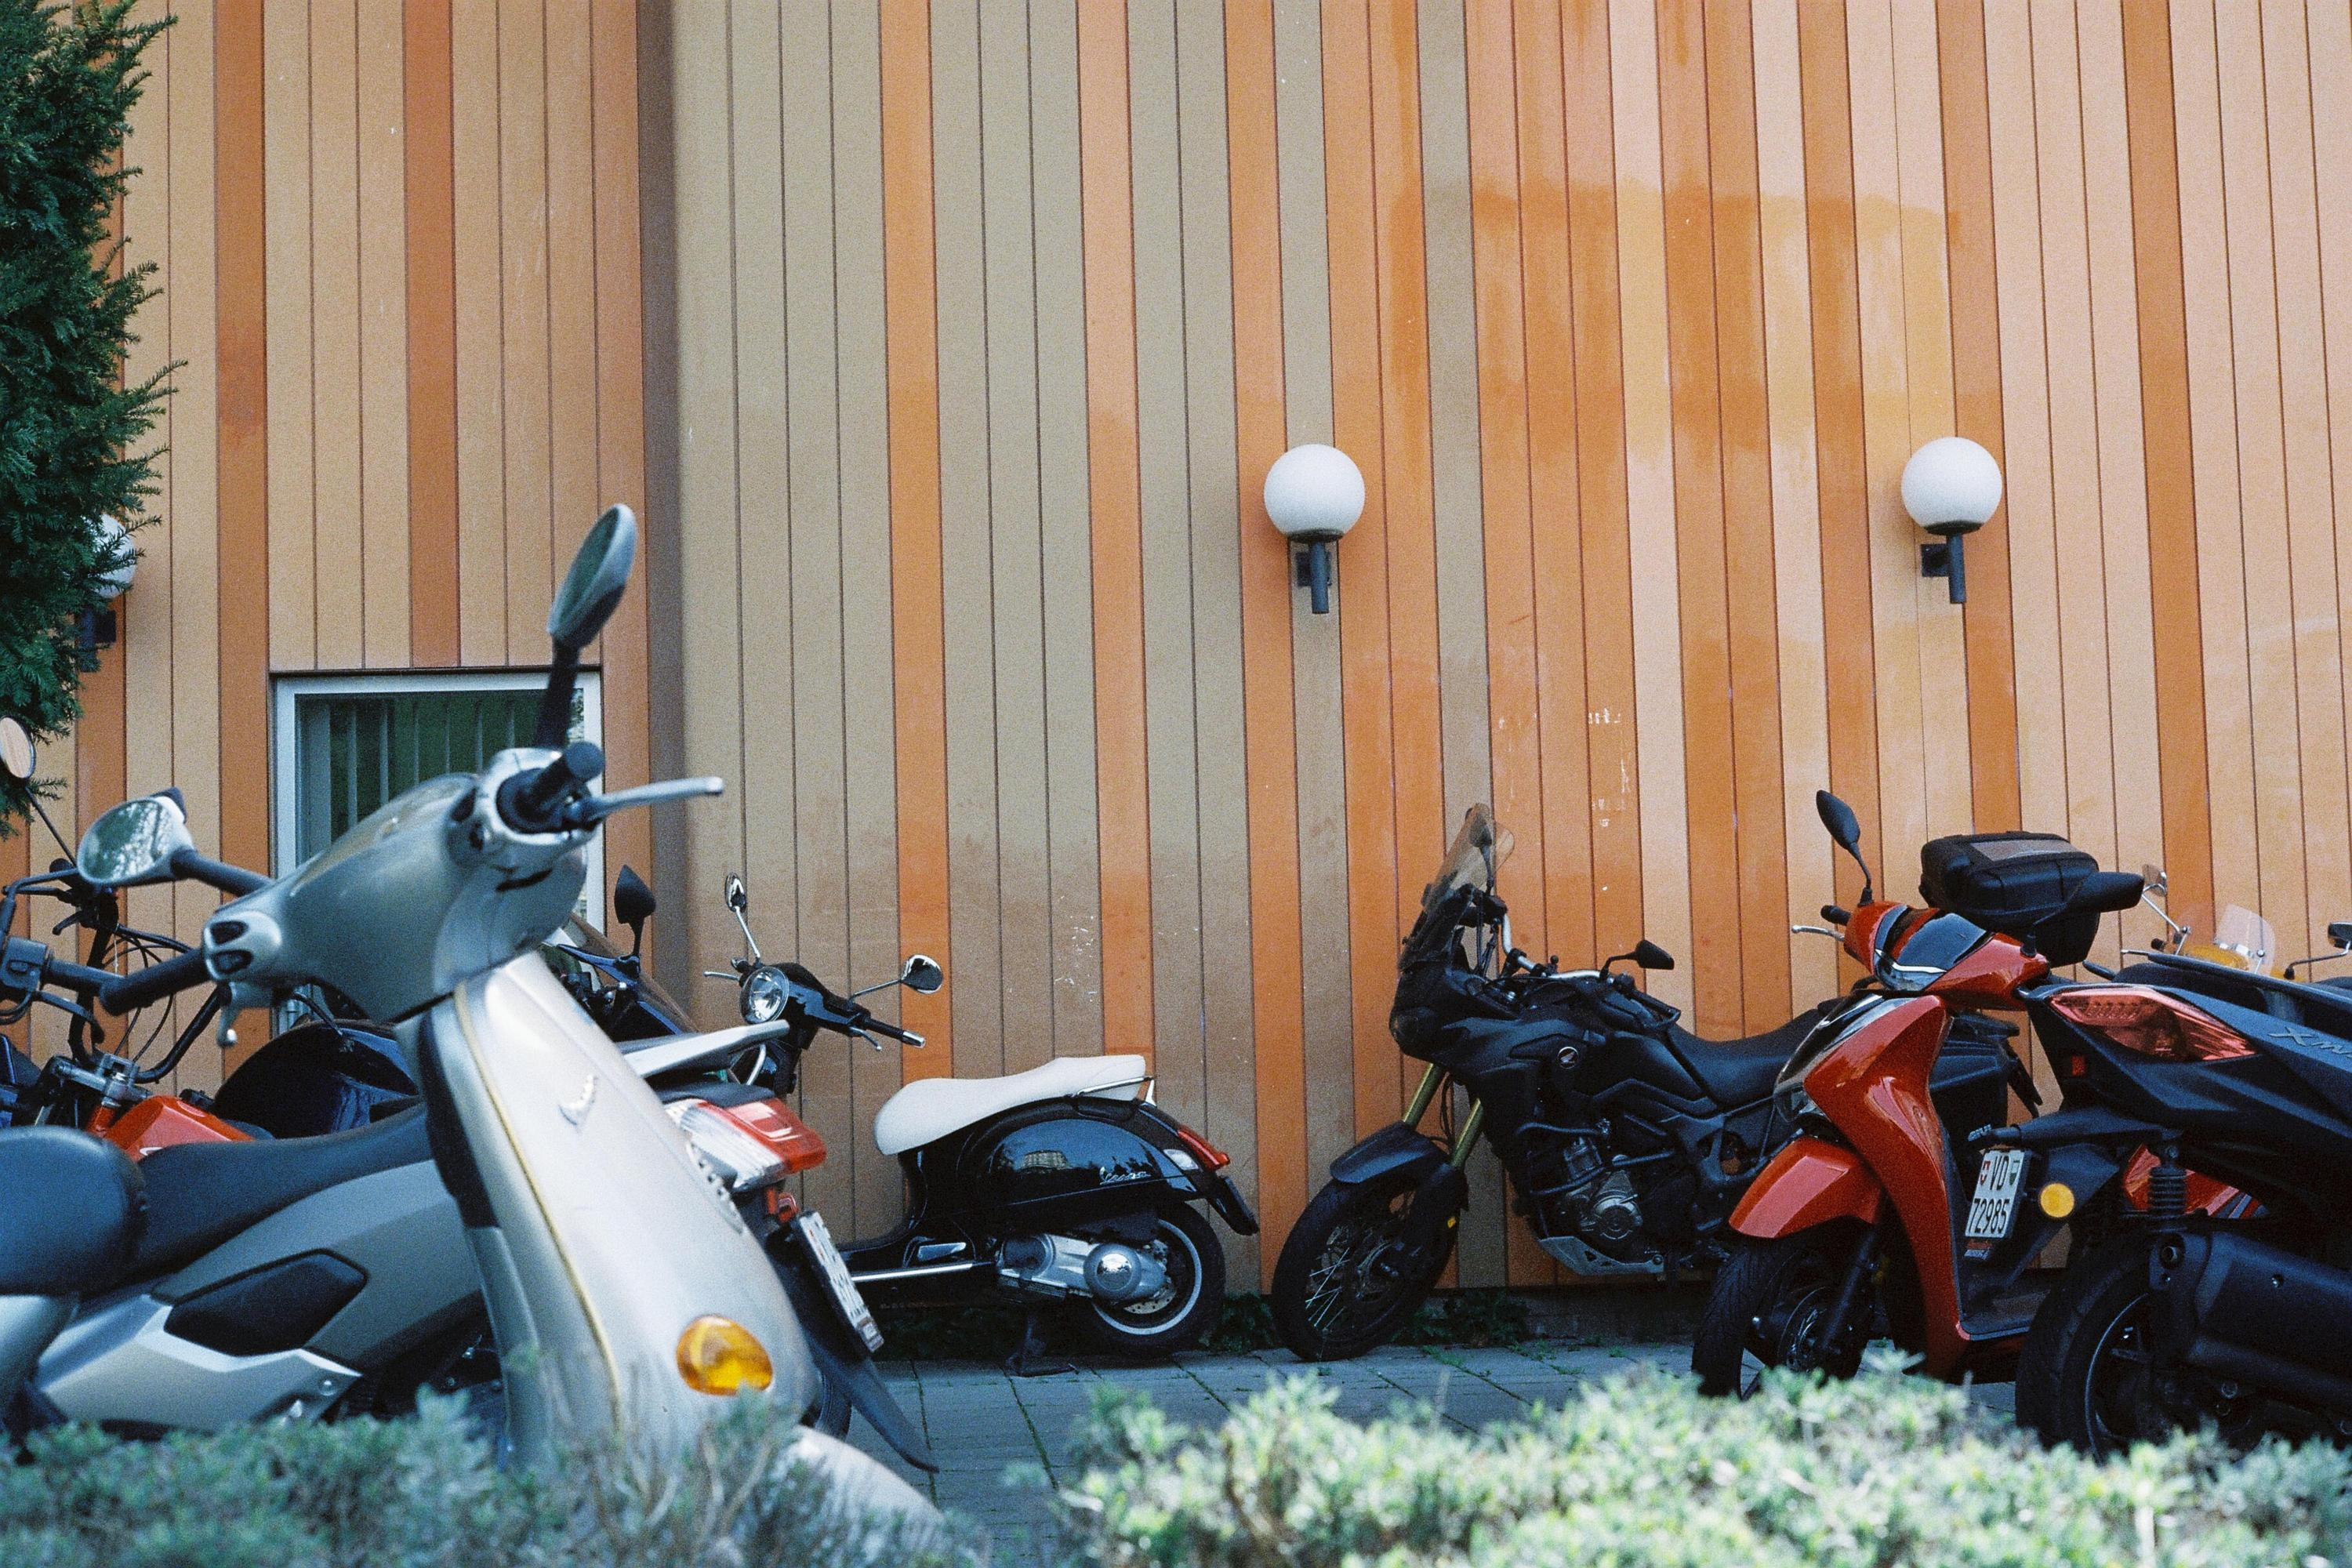
\includegraphics[width=\linewidth]{figures/film4.jpeg}
      \caption{Pair 4}
    \end{subfigure}
    \begin{subfigure}[t]{.19\textwidth}
      \centering
      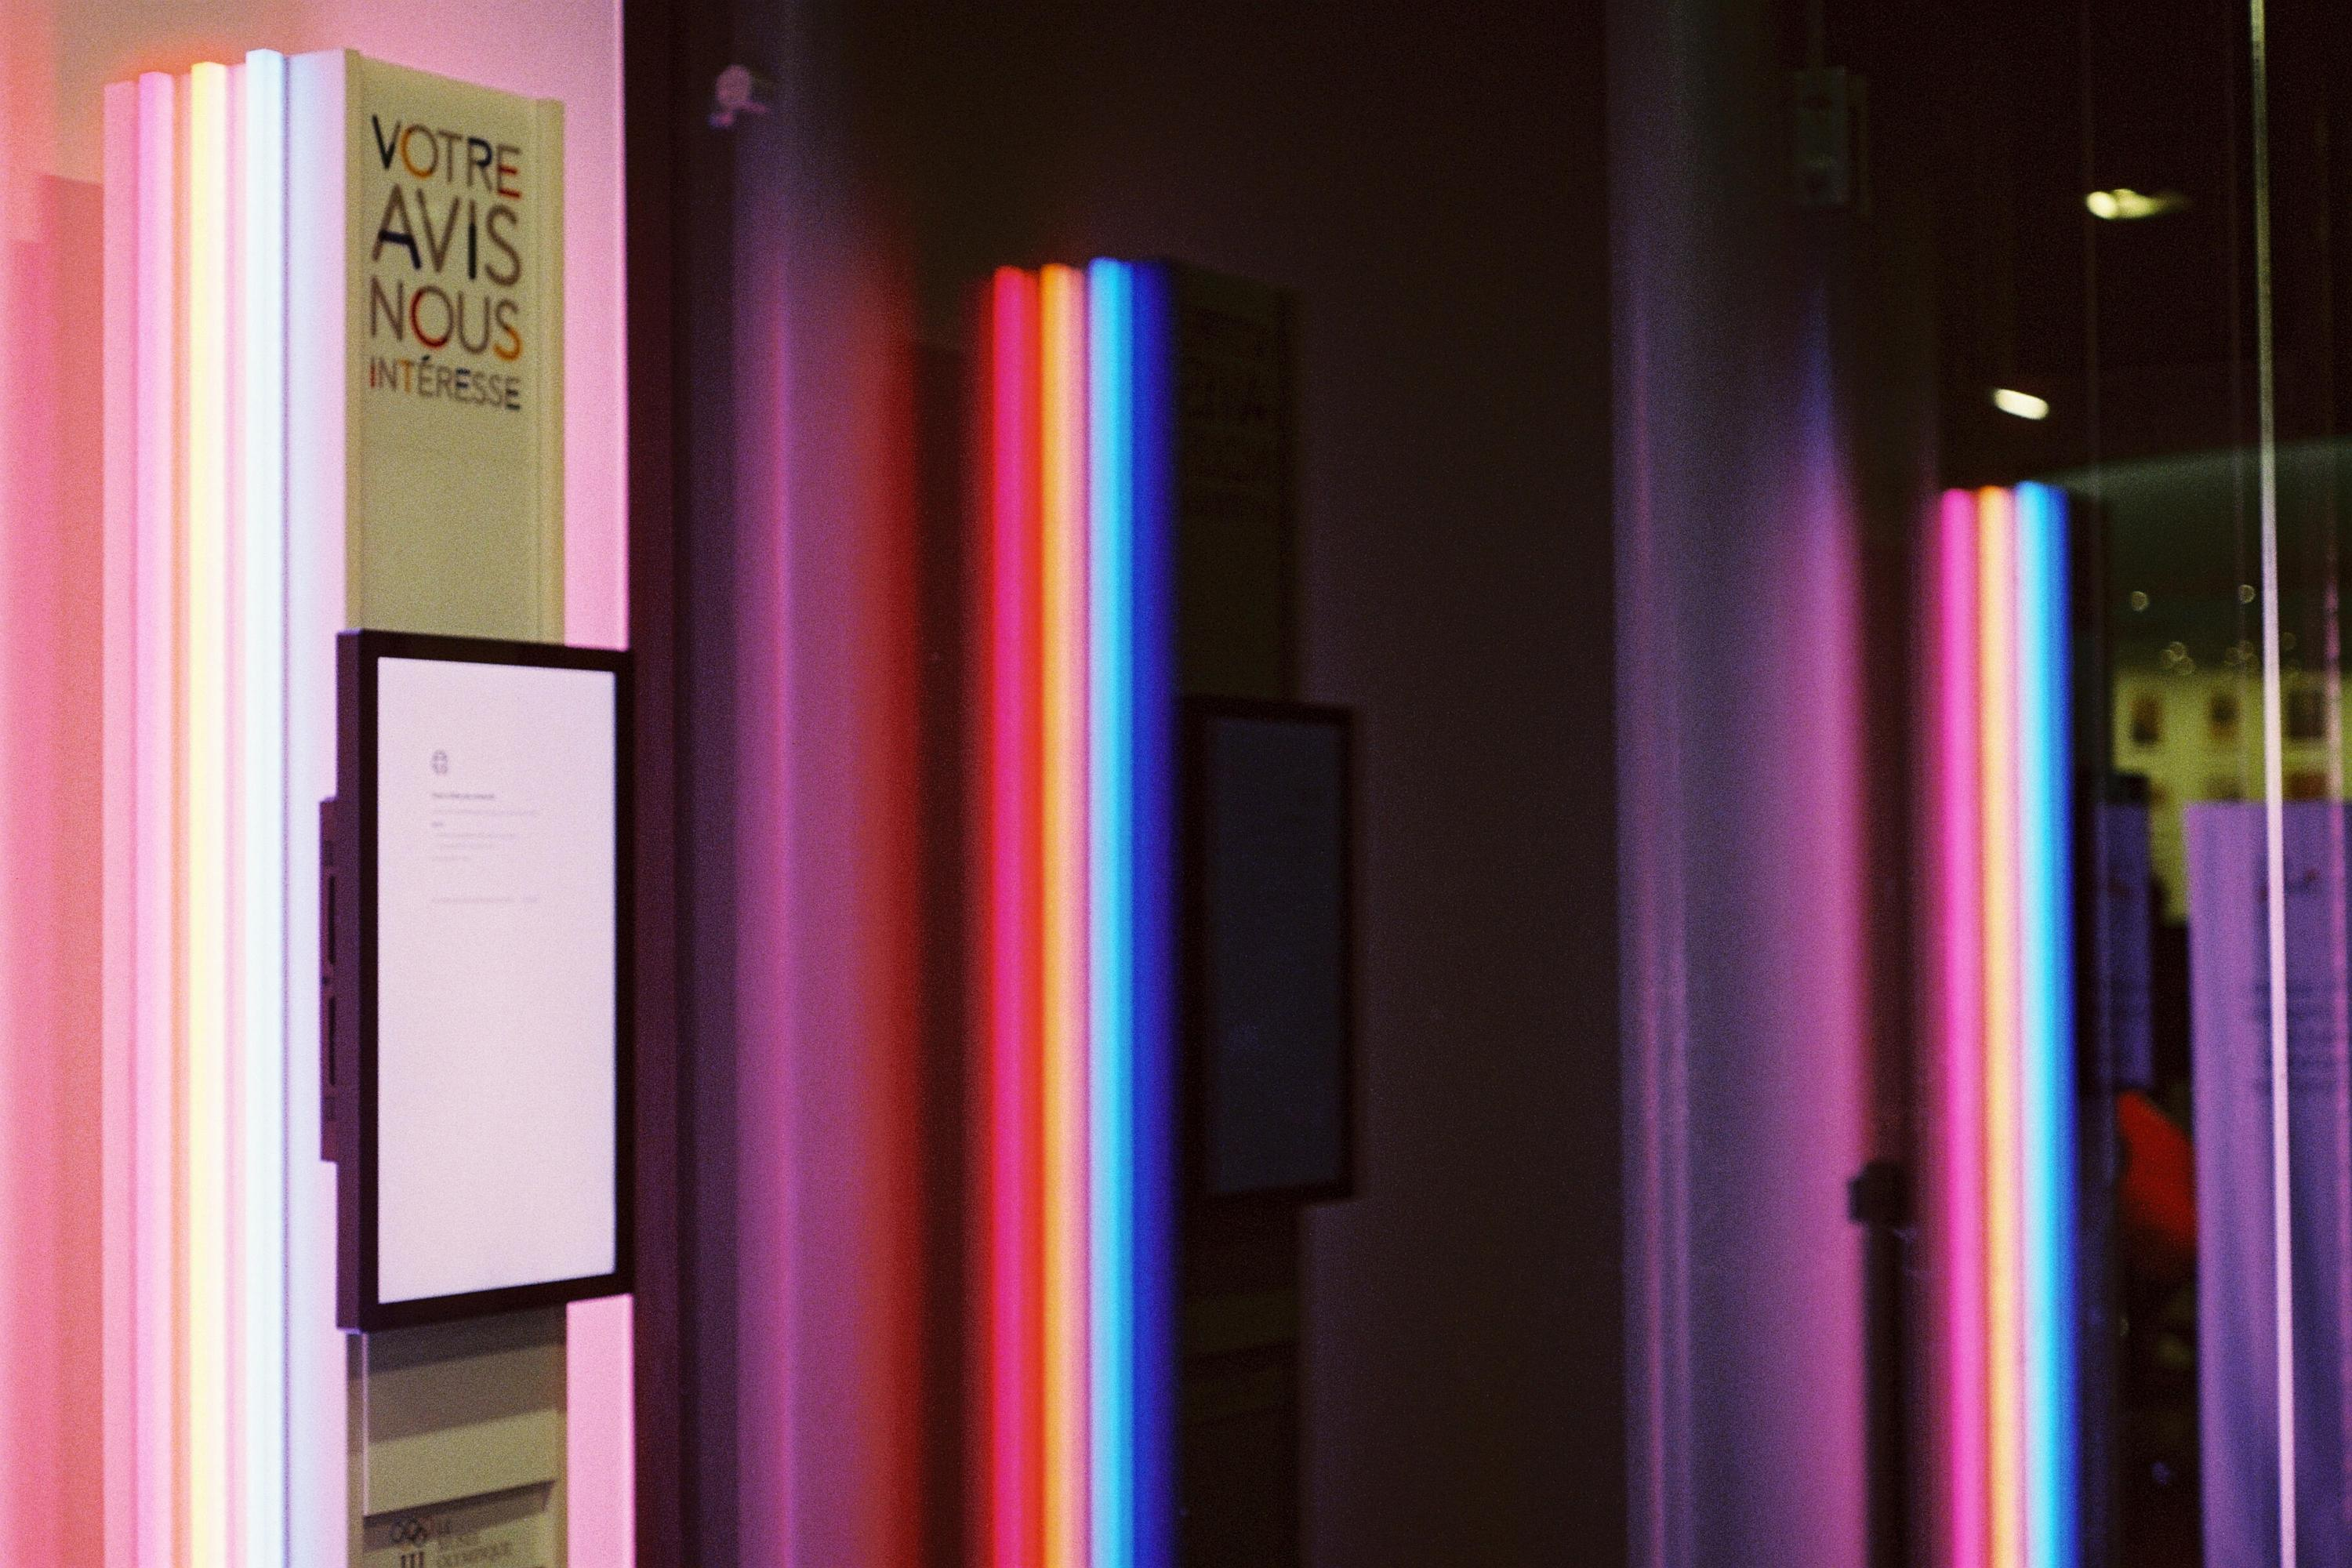
\includegraphics[width=\linewidth]{figures/film5.jpeg}
      \caption{Pair 5}
    \end{subfigure}
  
    \caption{\textbf{Raw Paired Image Dataset.} Examples of raw image pairs from the dataset. A column shows a single scene captured with a digital camera (top) and a film camera (bottom). The images show a wide range of scenes and visual effects.}
    \label{fig:raw-dataset}
\end{figure}

\subsubsection*{Data Preprocessing}
\label{subsubsec:preprocessing}

Due to the differences in the capturing process, the digital and film images
were not perfectly spatially aligned and showed different dynamic ranges. We
performed a series of pre-processing steps to address these issues. 

% Keypoint Alignment
irst, we aligned the images using keypoint alignment. This technique is based on the assumption that the digital and film images should contain the same visual features. We follow a standard image processing pipeline using openly available implementations of common feature detection, matching and perspective transformation algorithms from the OpenCV library~\cite{opencv}. For all image pairs we perform the following steps:

\begin{enumerate}
    \item \textbf{Keypoint Detection} We use the ORB~\cite{orb} (Oriented FAST and Rotated BRIEF) feature detection algorithm to detect keypoints and extract descriptors from both images.
    \item \textbf{Keypoint Matching} We then use the FLANN~\cite{flann} (Fast Library for Approximate Nearest Neighbors) algorithm to match the keypoints between the images. We apply the Lowe's ratio test to filter out matches that are likely to be incorrect.
    \item \textbf{Homography Estimation} Finally, we estimate a homography matrix using a subset of the matched keypoints using the RANSAC algorithm~\cite{ransac}. The matrix defines a perspective transformation which we apply to the digital image to align it with the film image.
\end{enumerate}

% TODO: Could go into more detail about the maths behind the algorithms and algorithms' parameters used in our experiments

% TODO: Could mention that we tried other keypoint detection algorithms: 
% We also experimented with other keypoint detection algorithms, such as SIFT (Scale-Invariant Feature Transform)~\cite{sift} and SURF (Speeded-Up Robust Features)~\cite{surf}, and simple brute-force feature matching algorithms, but found that the above pipeline provided accurate results and did not require a patent license.

% Luminance Alignment
Next, we address the differences in the dynamic range of the images. To ensure that our model does not learn systematic brightness adjustments caused by slight variations in the camera setup during our data collection, we aimed to align the luminance of the film image to the digital image. In this way, the digital image serves as a reference for the luminance of the film image, as we want our training distribution to be as close as possible to the types of images our model will see at inference time. The luminance alignment is performed using histogram matching in CIELAB space. Specifically, we follow these steps:

\begin{enumerate}
    \item \textbf{Convert to CIELAB} We convert both the digital and film images to the CIELAB colour space. This colour space is designed to approximate human vision and is more perceptually uniform than the RGB colour space. Crucially, the luminance channel $L$ is separated from the chrominance channels $a$ and $b$ which allows us to focus on the luminance information.
    \item \textbf{Histogram Matching} We then match the luminance histogram of the film image to the digital image. This is done by computing the cumulative distribution function (CDF) of the luminance channel of both images and then performing a linear interpolation to map the luminance values of the film image to the digital image.
    \item \textbf{Convert back to RGB} Finally, we convert the film image back to the RGB colour space.
\end{enumerate}

We observe that both the keypoint alignment and luminance matching steps are
crucial prerequisites for training our model. An example of the results of these
steps can be seen in Figure~\ref{fig:data-preprocessing}. After the
preprocessing steps we are left with 38 processed image pairs (three images
could not be aligned) which we refer to as $D_{\text{processed}}=\{(I^F_n,
I^D_n)\}_n^{38}$. We publicly release both the raw and processed dataset to
facilitate further research in this or related areas.

\begin{figure}
    \begin{subfigure}[t]{.49\textwidth}
      \centering
      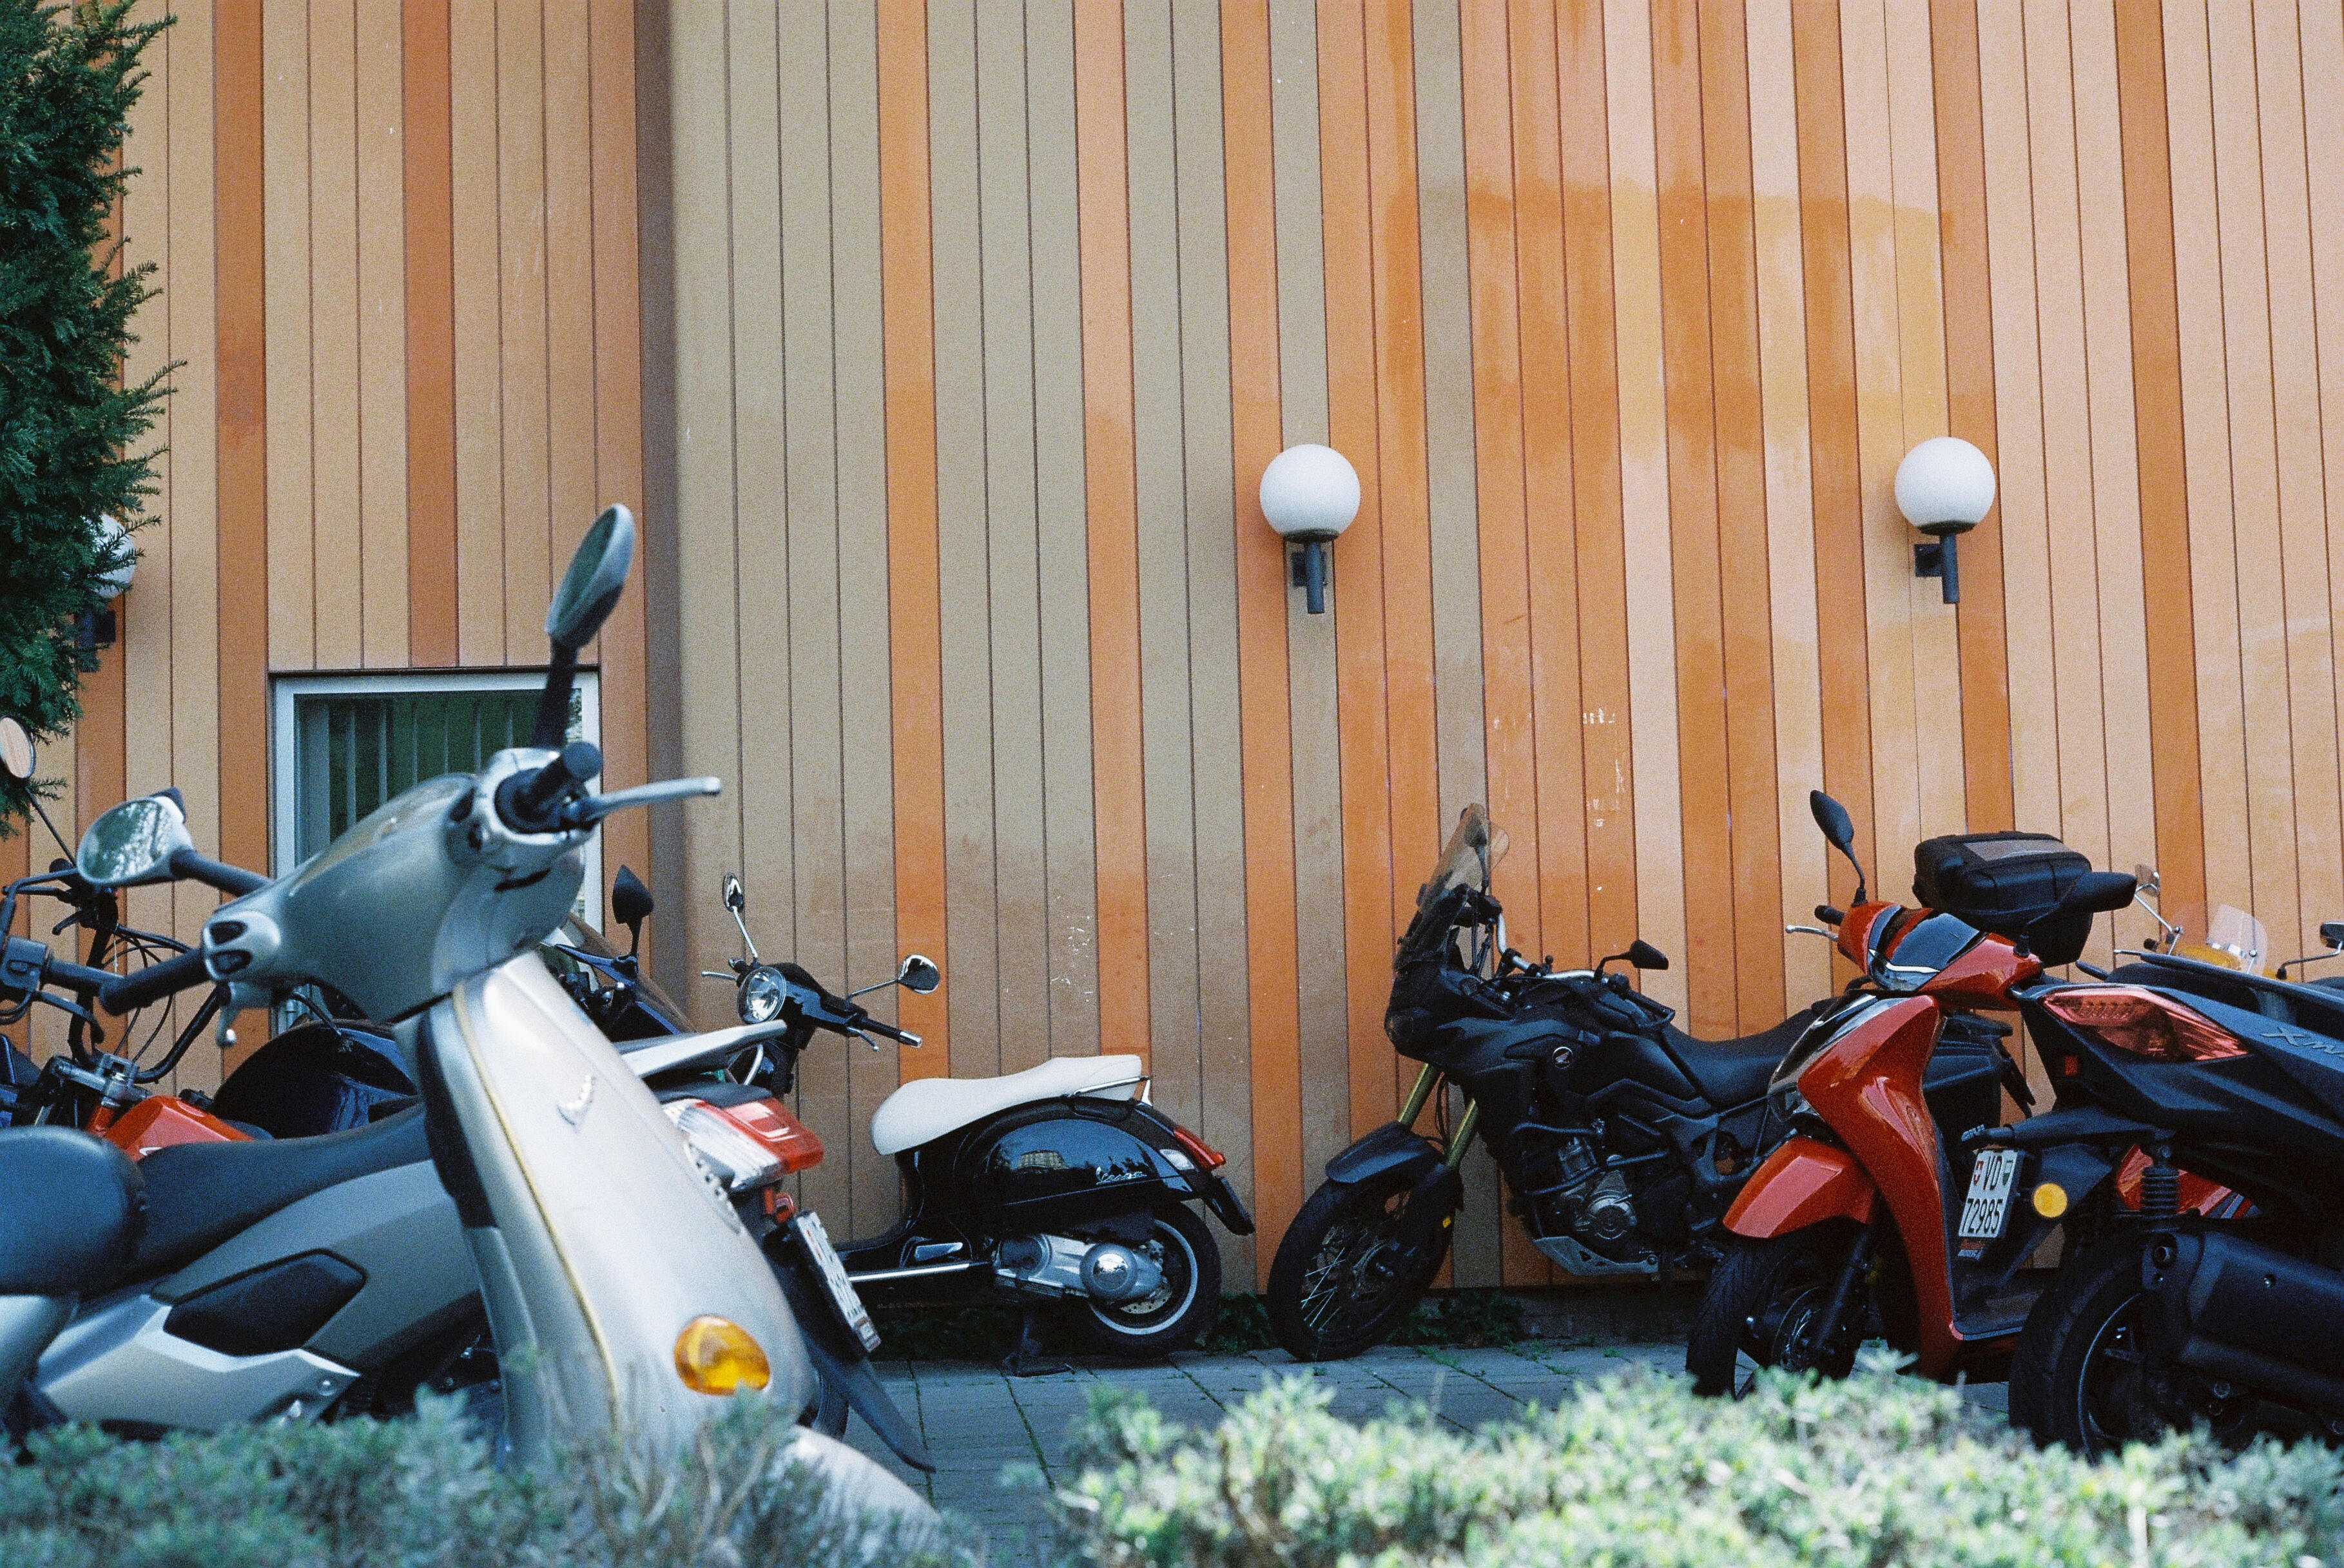
\includegraphics[width=\linewidth]{figures/raw-film.jpeg}
      \caption{Raw Film Image}
    \end{subfigure}
    \hfill
    \begin{subfigure}[t]{.49\textwidth}
      \centering
      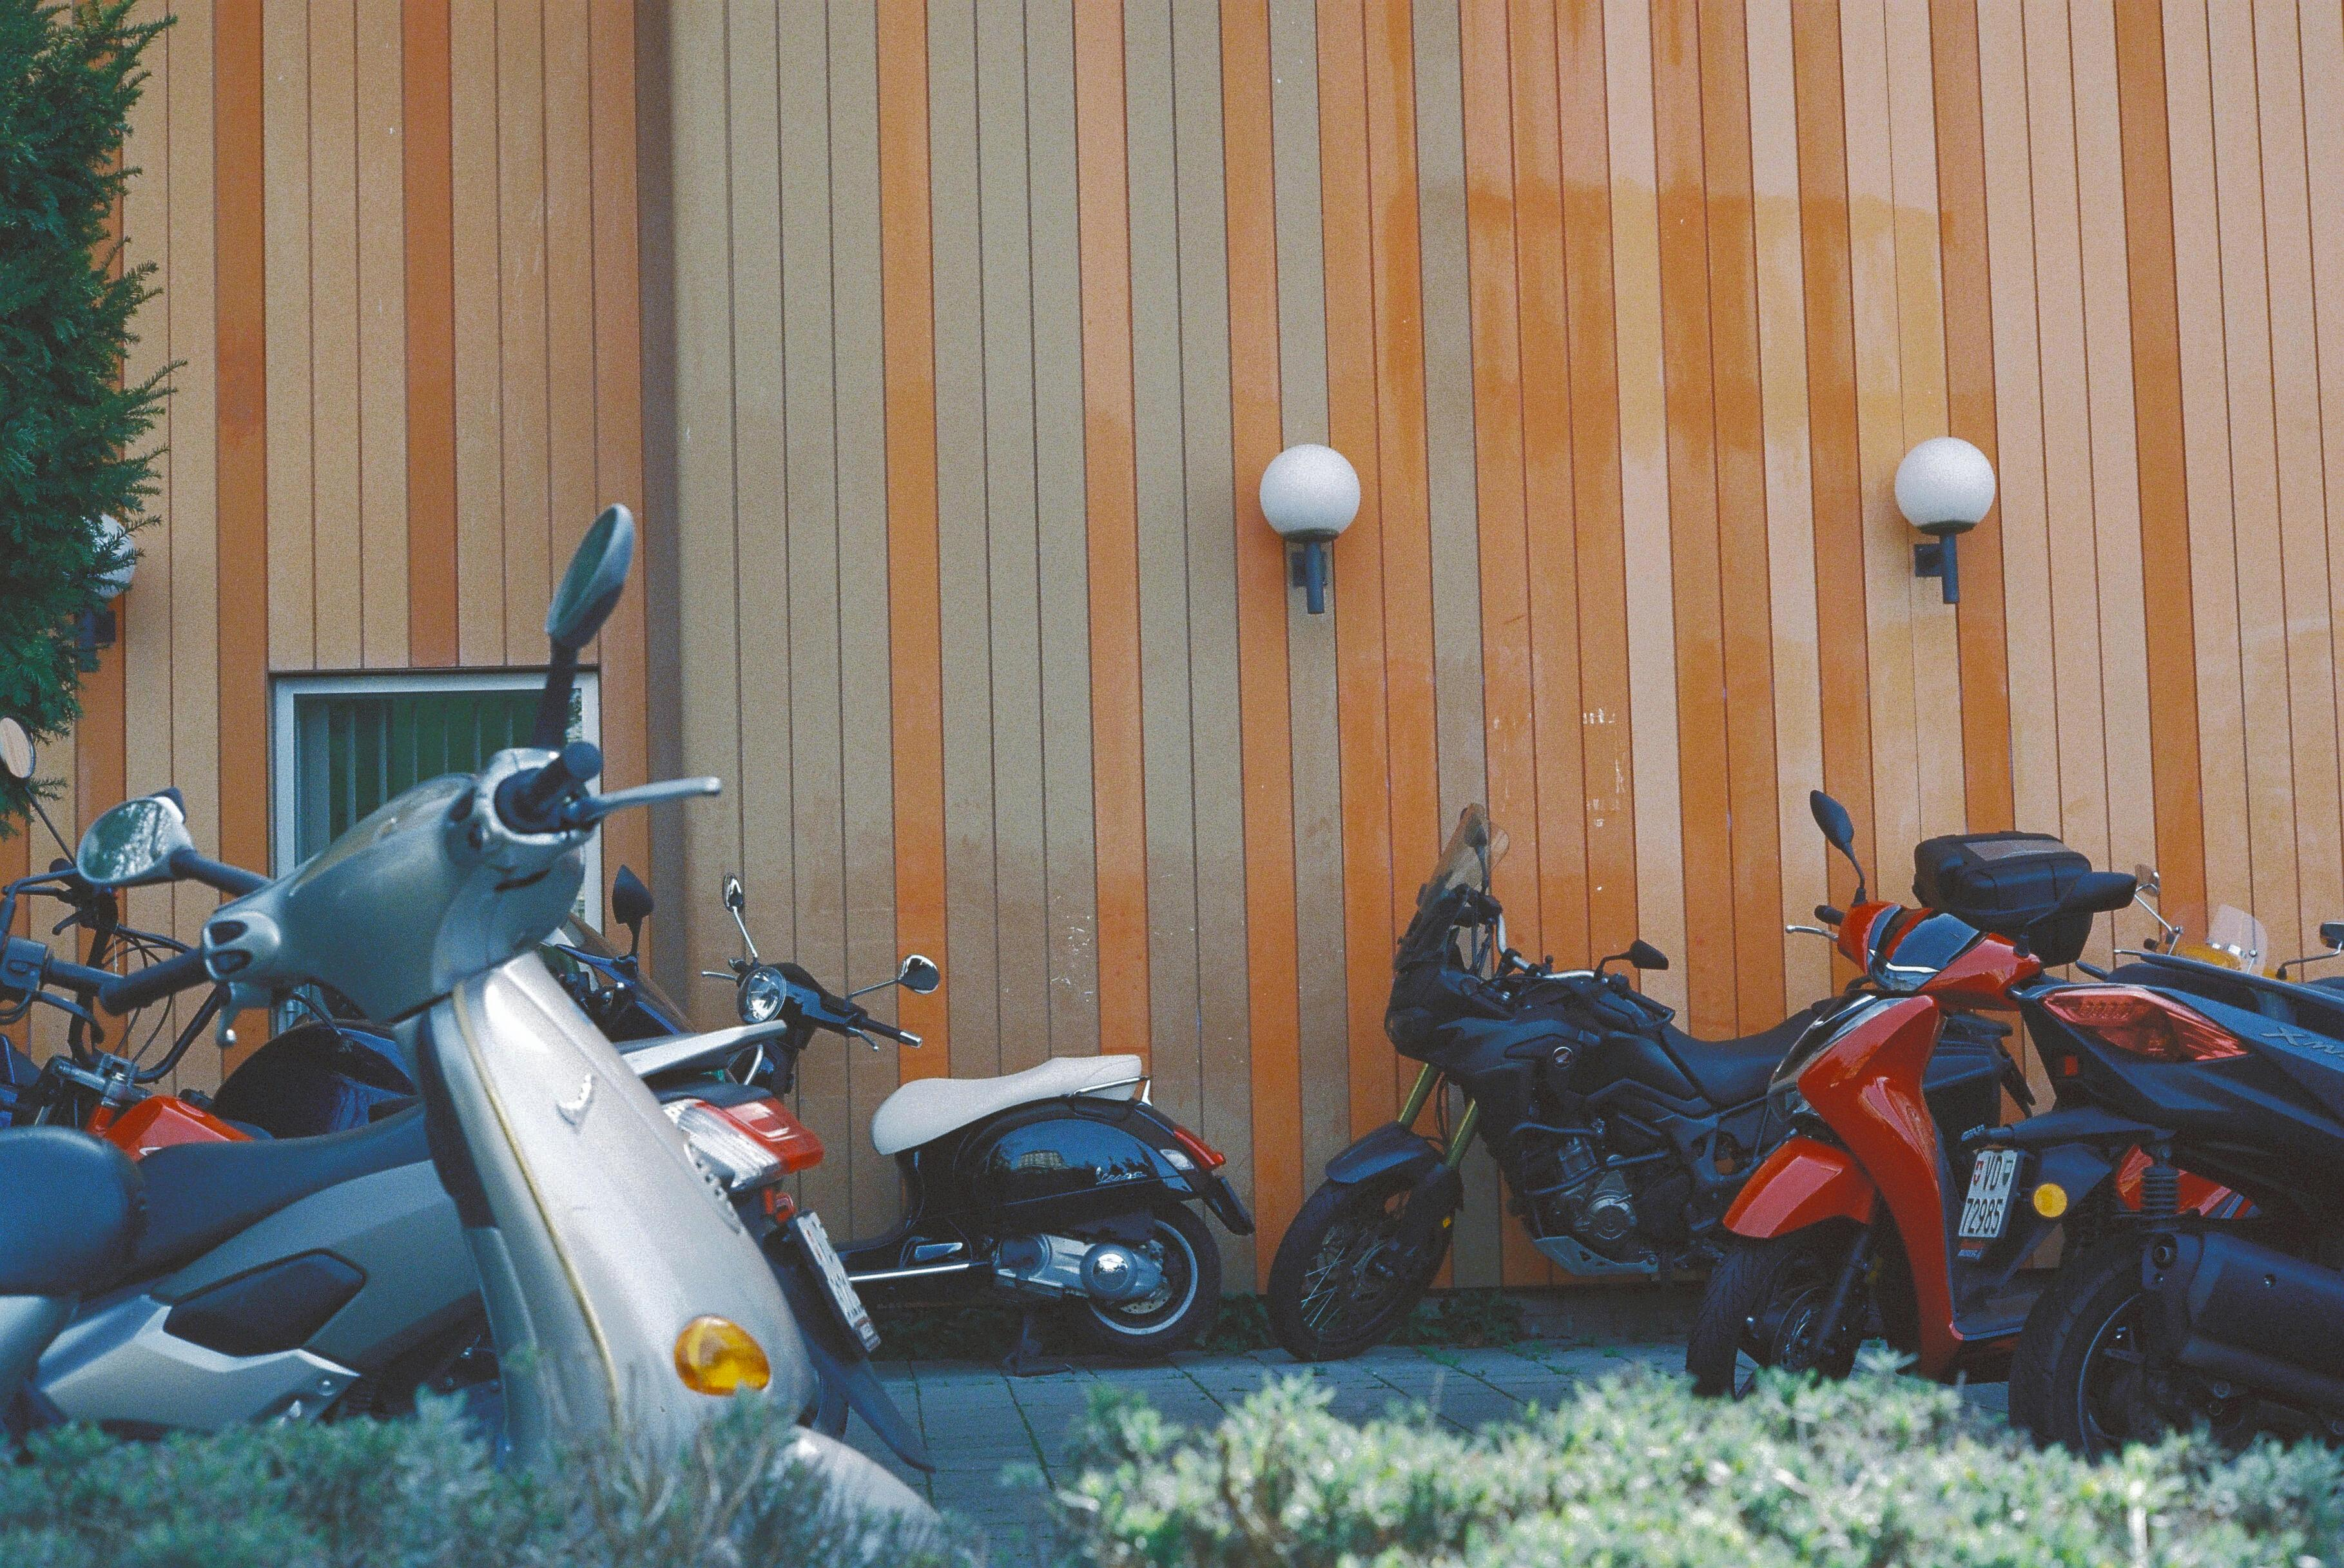
\includegraphics[width=\linewidth]{figures/processed-film.jpeg}
      \caption{Processed Film Image}
    \end{subfigure}
  
    \medskip
  
    \begin{subfigure}[t]{.49\textwidth}
      \centering
      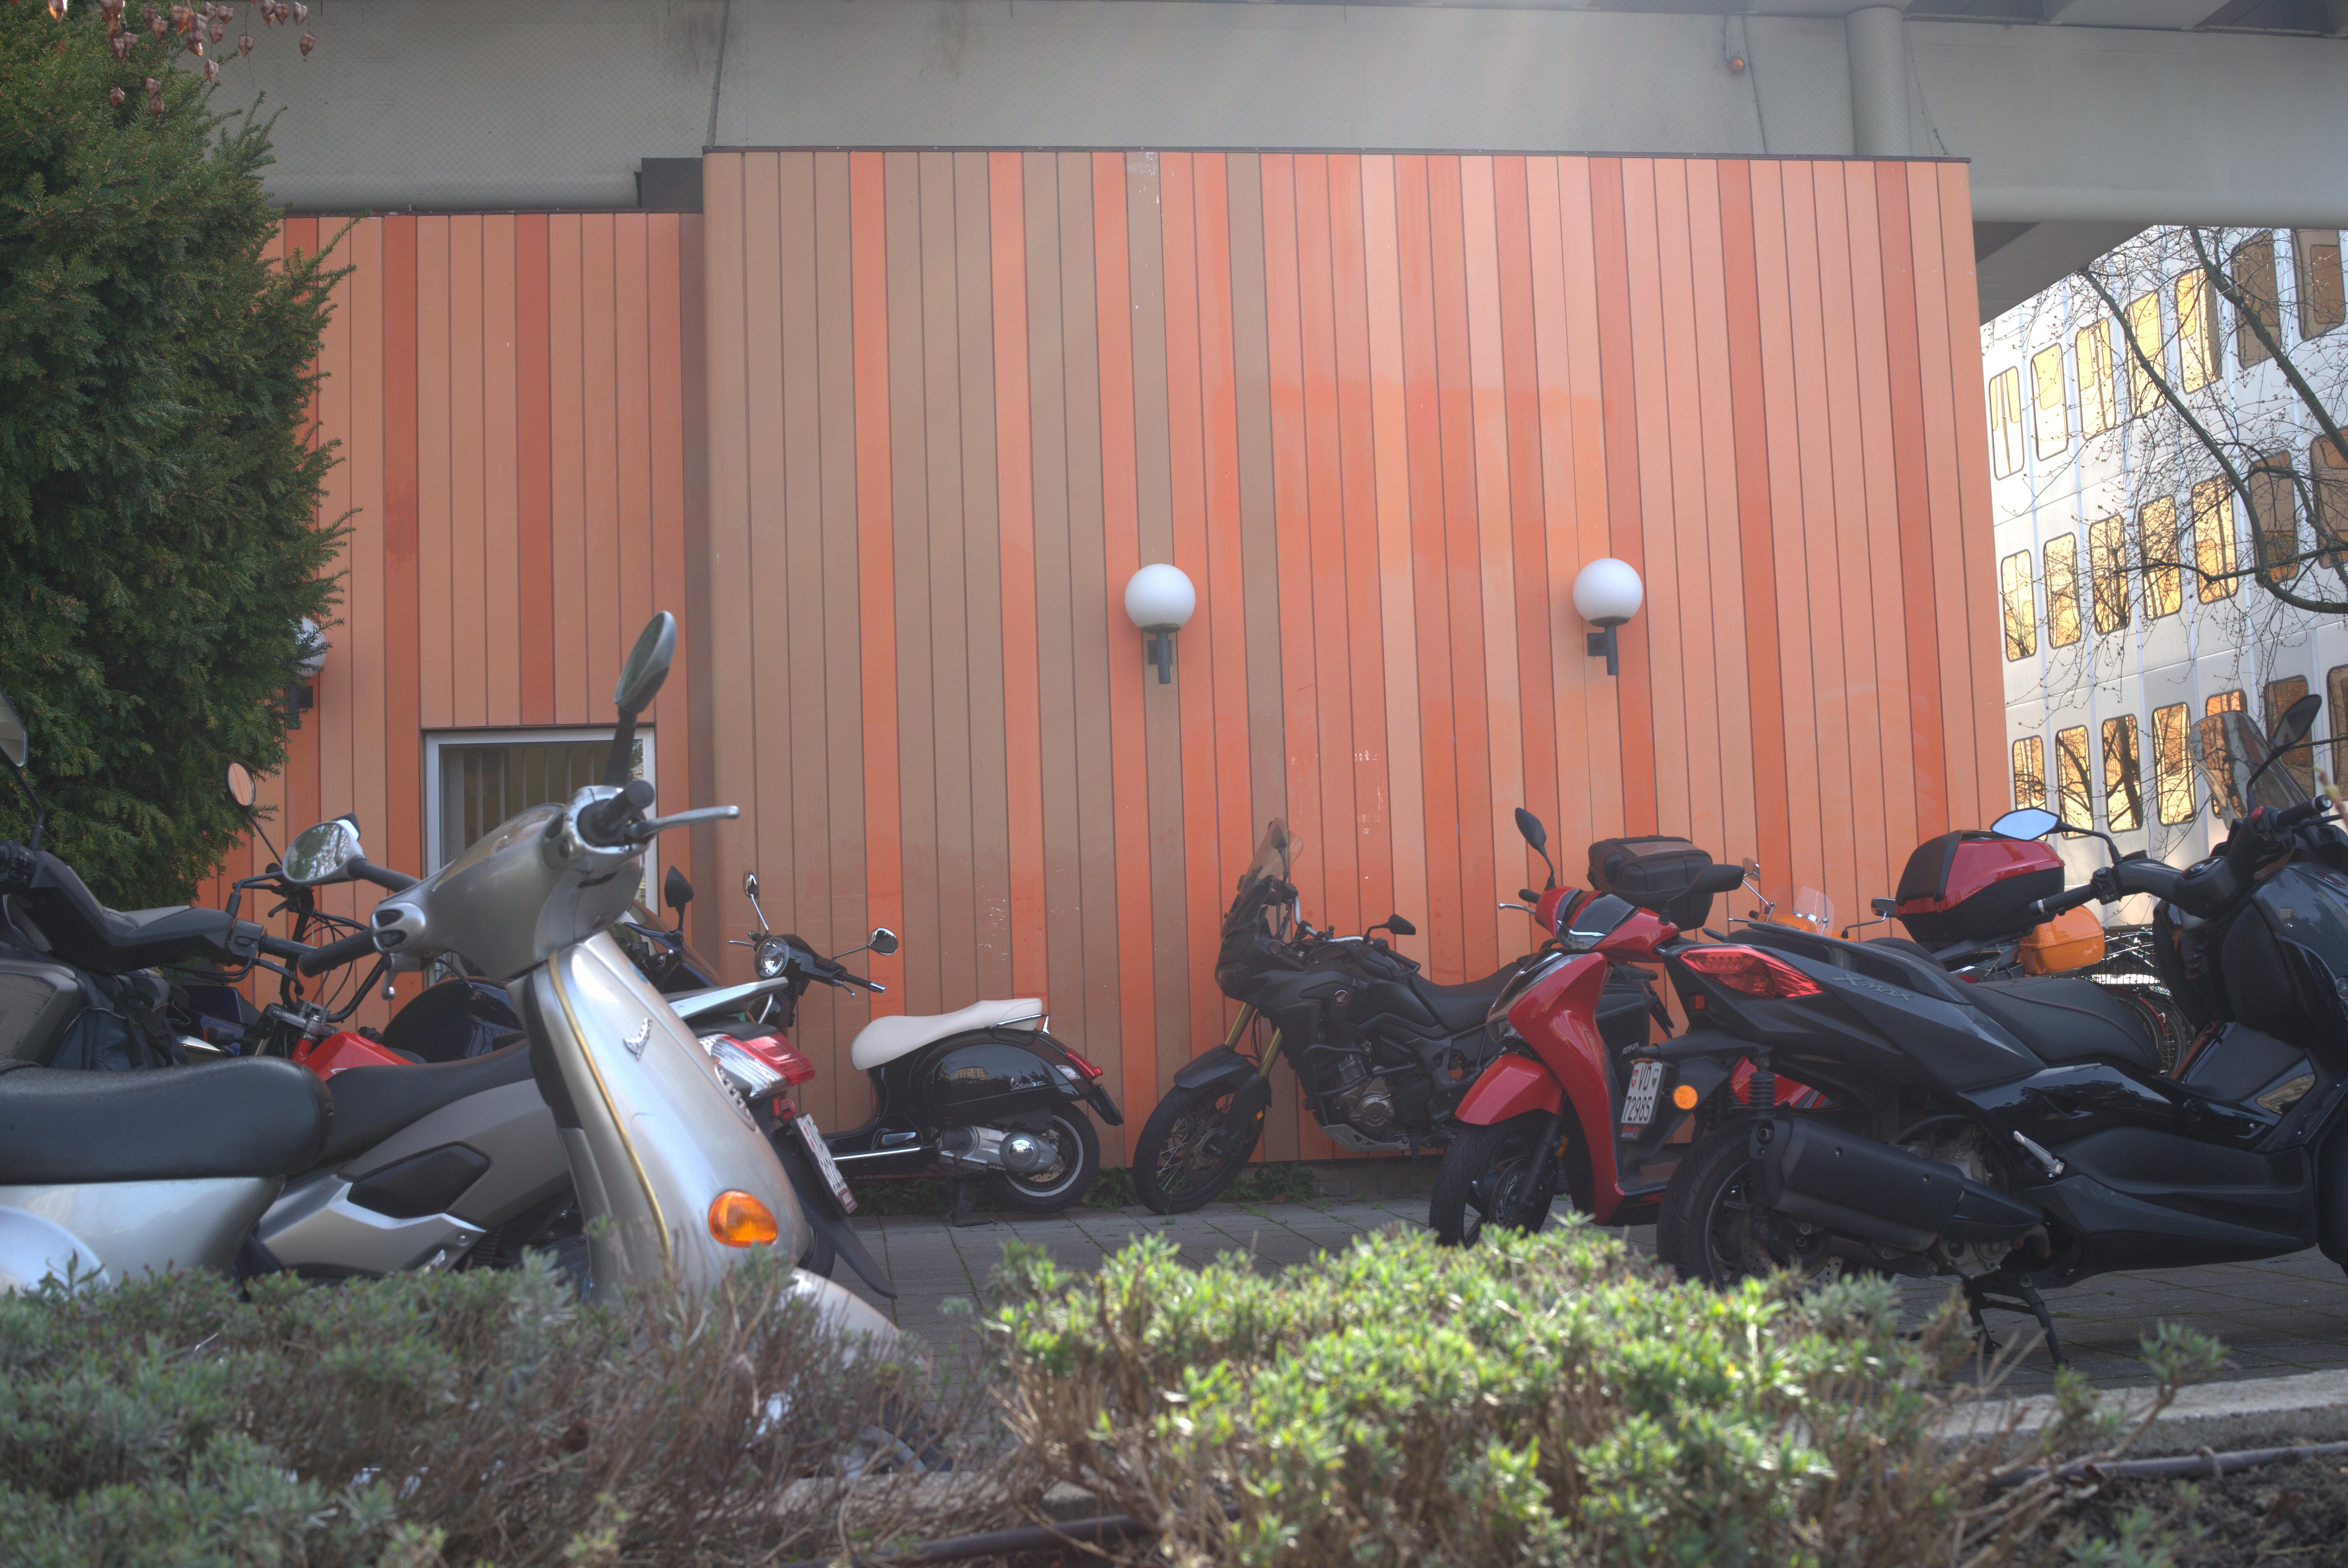
\includegraphics[width=\linewidth]{figures/raw-digital.jpeg}
      \caption{Raw Digital Image}
    \end{subfigure}
    \hfill
    \begin{subfigure}[t]{.49\textwidth}
      \centering
      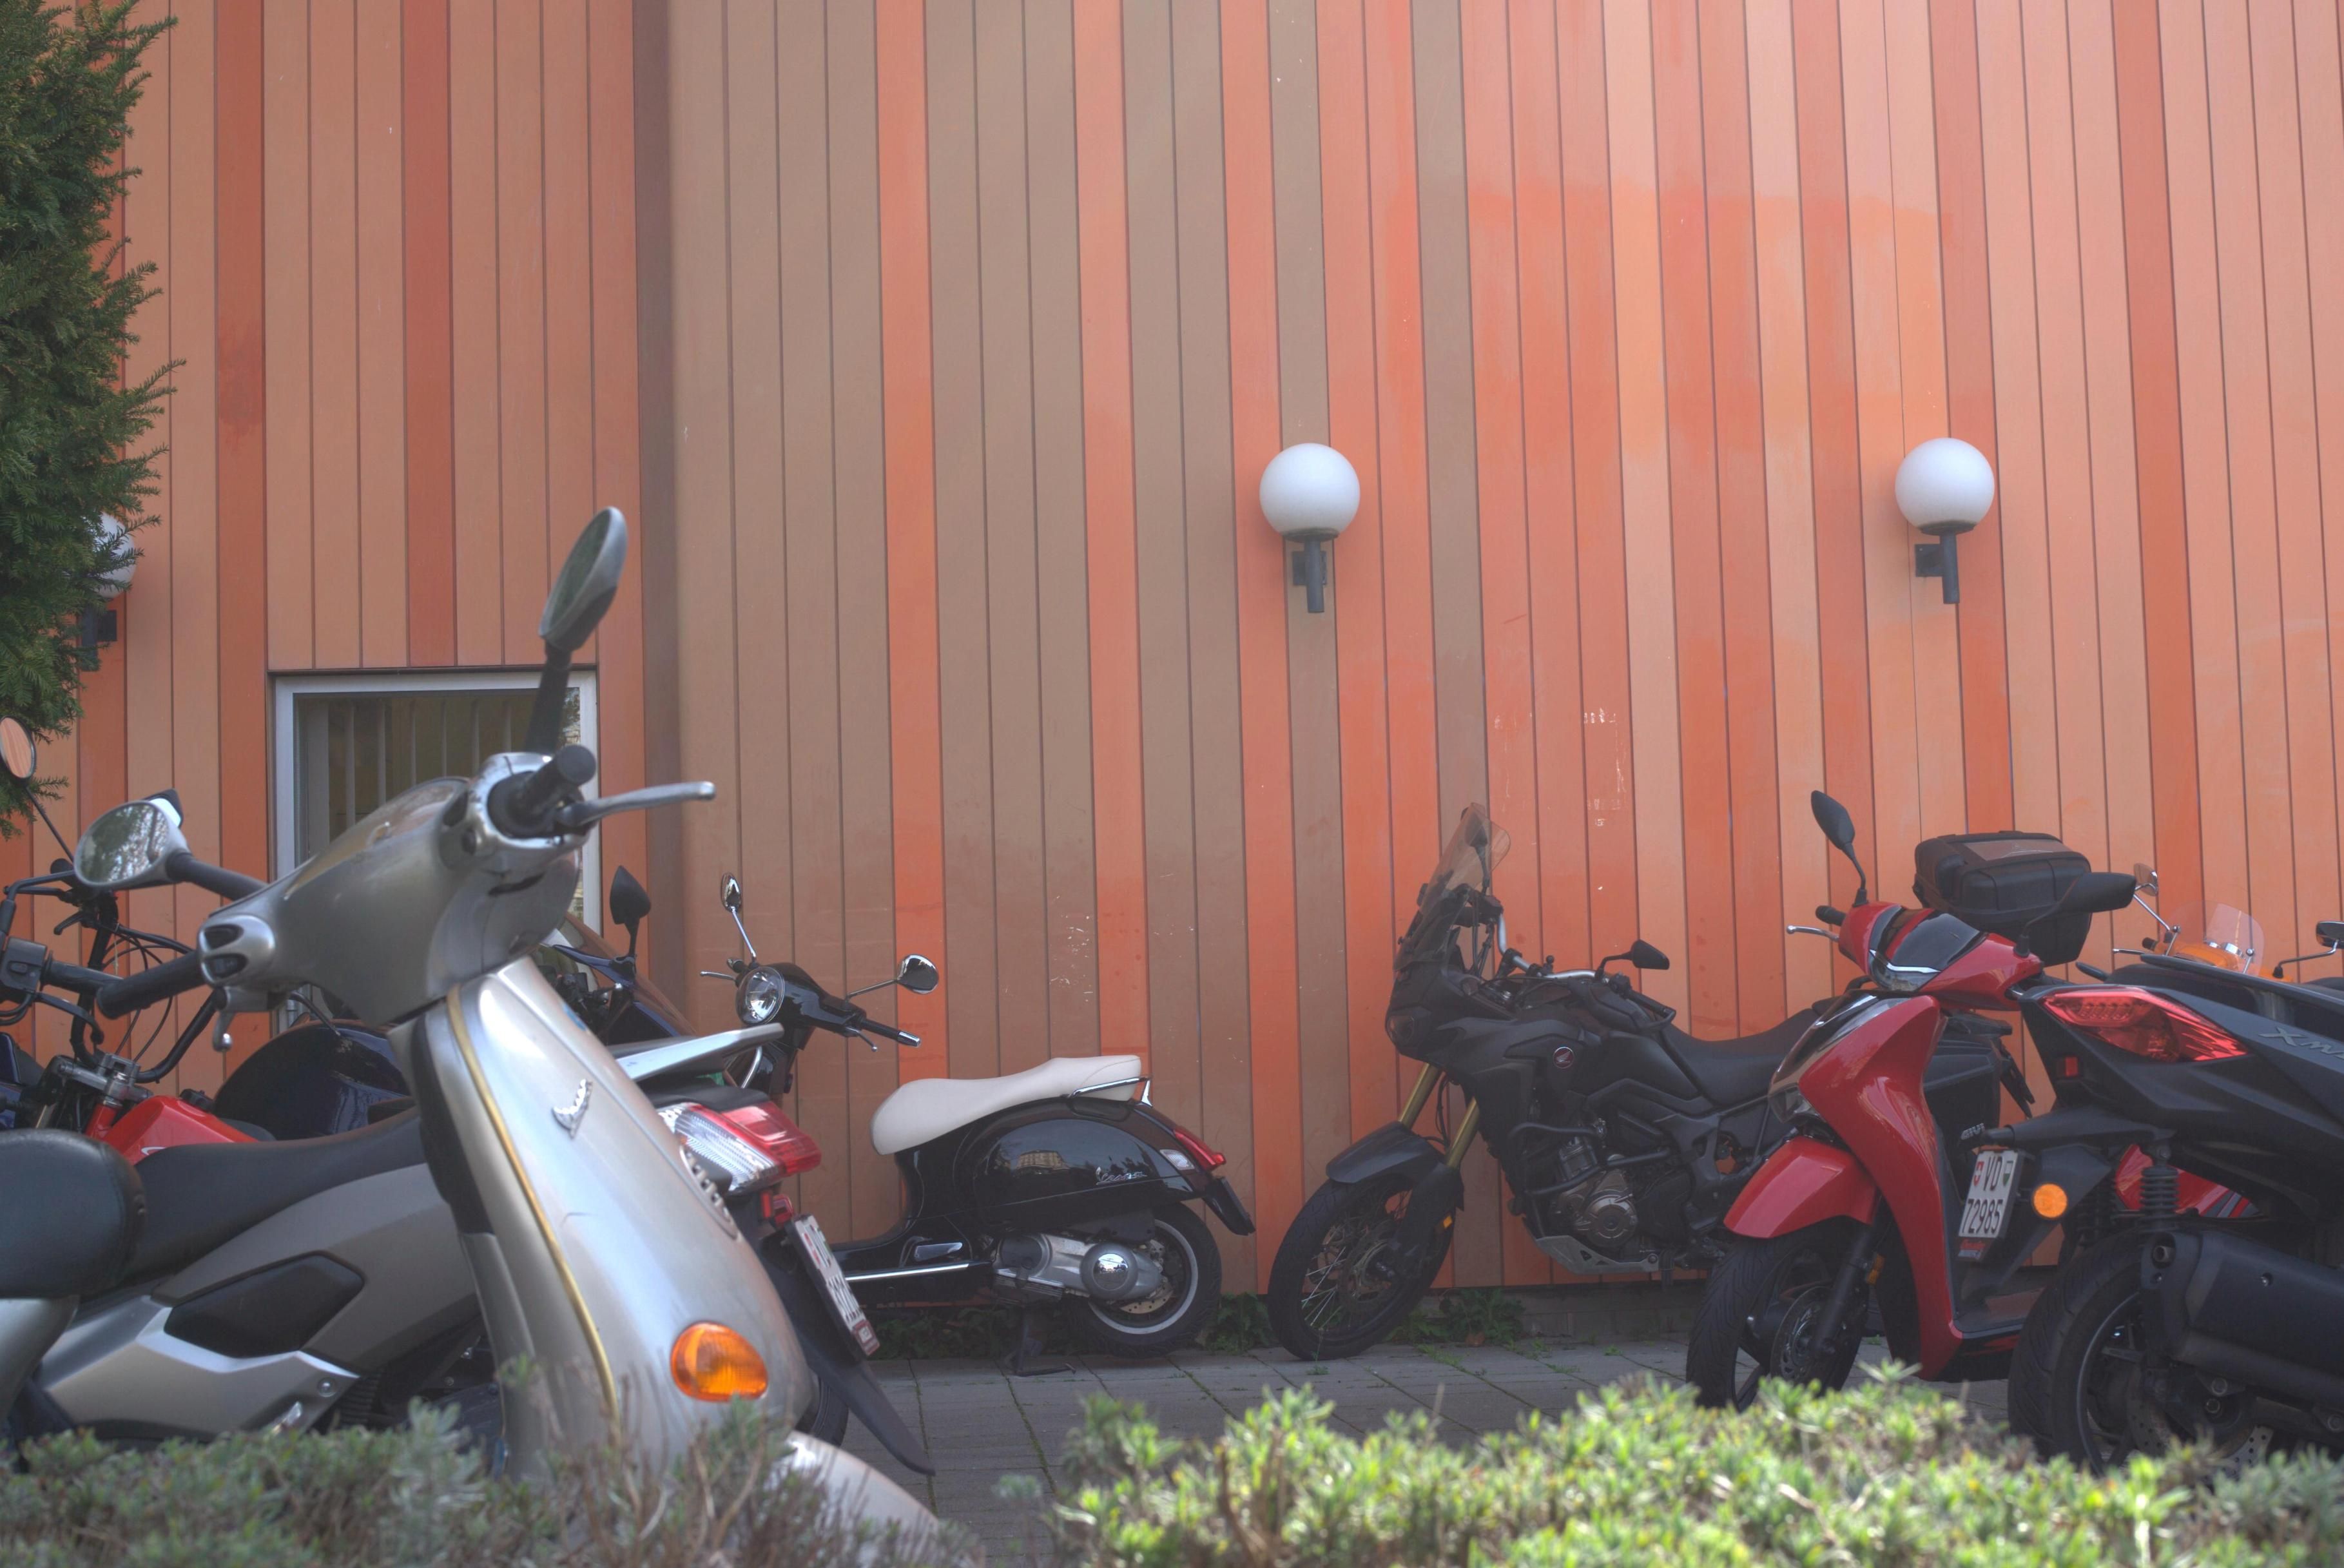
\includegraphics[width=\linewidth]{figures/processed-digital.jpeg}
      \caption{Processed Digital Image}
    \end{subfigure}

    \caption{\textbf{Dataset Preprocessing.} Example of a raw and processed image pair. The raw images (a) and (c) show misalignment and differences in dynamic range. After keypoint alignment and luminance matching, the processed images (b) and (d) are spatially and luminance aligned.}
    \label{fig:data-preprocessing}
\end{figure}

For our experiments we consider training both on single-image datasets and on the full dataset. The single-image datasets are created by manually selecting an image from the full dataset that best represents a specific visual effect, like graininess or colour cast. For such datasets, we train and evaluate the model on the same image to ensure that the model learns the desired effect. The full dataset is used to train a model that can generalize to a wide range of visual effects, and is split into a training, validation and test split according to the guidelines in Section~\ref{subsec:training}.

% TODO: Maybe talk about data augmentation (horizontal/ vertical flips, brightness adjustment and blur)

% TODO: Add figure of example pair before and after pre-processing


\subsection{Model}
\label{subsec:model}

All of our experiments are based on model architectures inspired by U-Net~\cite{unet}. U-Net is a type of convolutional neural network (CNN) architecture that was originally designed for image segmentation tasks and has since been adapted for various image-to-image translation tasks. The U-Net architecture consists of a contracting path (encoder) and an expansive path (decoder) with skip connections between them. The encoder path consists of stacked convolutional blocks with alternating convolutional layers and non-linear activation functions followed by a 2x2 max pooling down-sampling. The decoder path consists of up-sampling layers followed by convolutional blocks with skip connections from the encoder path. The skip connections help to preserve detailed information from the input image and have been shown to improve the performance of the model. 

For our experiments we vary the number of layers $L$, the number of filters $F$, and the kernel size $K$. All other parameters, such as zero-padding, the pooling and up-sampling operations, and the activation functions, are kept constant. No normalisation layers or dropout layers are used in the model.

\subsection{Loss Functions}
\label{subsec:loss-functions}

\textbf{Mean Squared Error Loss.} The mean squared error (MSE) loss is a common loss function used in image-to-image translation tasks. It measures the average squared difference between the predicted and ground truth images. For two images $I$ and $J$ of the same size, the MSE loss is defined as:

\begin{equation}
    \text{MSE}(I, J) = \frac{1}{n} \sum_{i=1}^{n} (I_i - J_i)^2
    \label{eq:mse}
\end{equation}

\textbf{Mean Absolute Error.} The mean absolute error (MAE) loss is another common loss function used in image-to-image translation tasks. It measures the average absolute difference between the predicted and ground truth images. For two images $I, J \in \mathbb{R}^{3 \times H \times W}$ the MAE loss is defined as:

\begin{equation}
    \text{MAE}(I, J) = \frac{1}{n} \sum_{c=1}^{3}\sum_{h=1}^{H} \sum_{w=1}^{W} |I_{c,h,w} - J_{c,h,w}|.
    \label{eq:mae}
\end{equation}

\textbf{VGG Loss.}

\textbf{Colour Loss.}

\textbf{Absolute Total Variational Loss.}

\textbf{Relative Total Variational Loss.}

\textbf{CoBi Loss.}

% TODO: Talk about combination of losses.

\subsection{Training}
\label{subsec:training}

% Optimiser: Adam w/ learning rate 1e-3
% Patched training
% Number of patches (instead of epochs)
% Batch size relatively small at 4

\begin{figure}
    \centering
    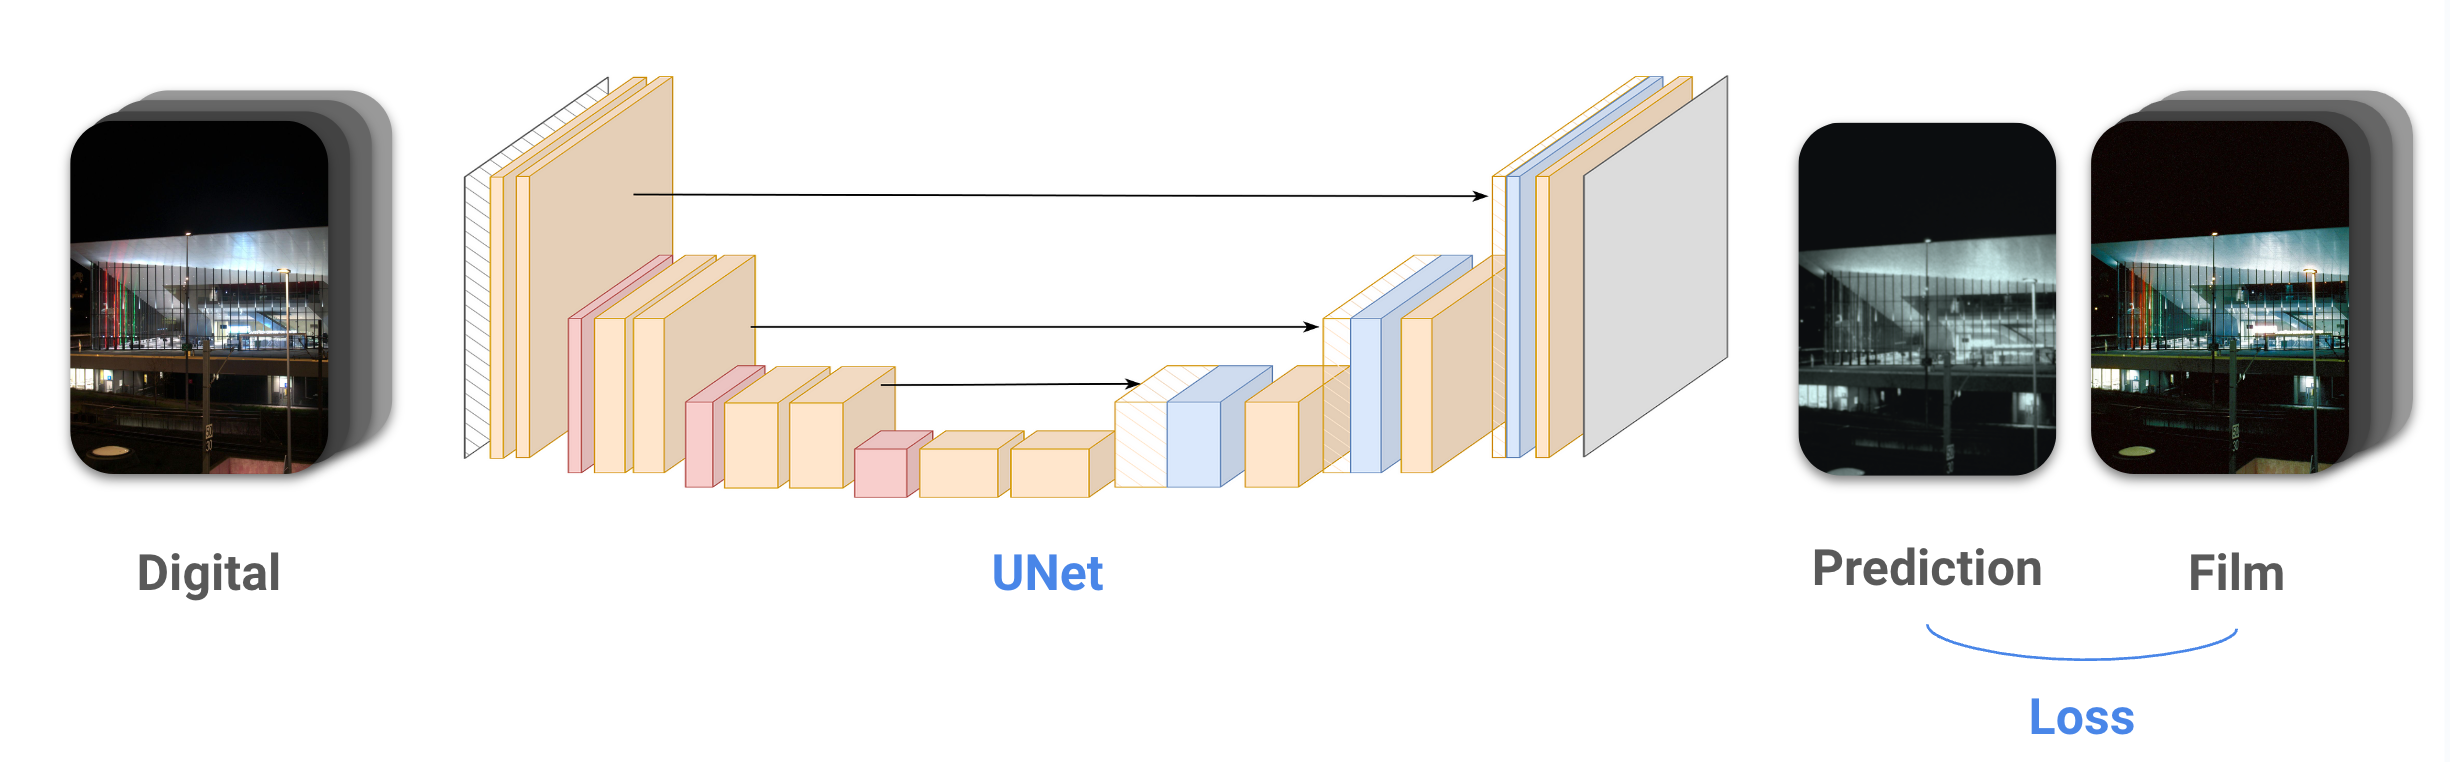
\includegraphics[width=0.9\textwidth]{figures/training-overview.png}
    \caption{\textbf{Training Overview.} We train our model on a dataset of paired digital-film images. The dataset is split into a training, validation and test set. The model is trained using the Adam optimizer with a learning rate of $1e-3$. We use a patched training approach, where the images are divided into patches of size $256 \times 256$ and the model is trained on these patches.}
    \label{fig:training-overview}
\end{figure}


\subsection{Evaluation}
\label{subsec:evaluation}

% Qualitative assessment: Visual comparison of results (patches during training/ evaluation + inference on downsampled images on full dataset)

% Quantitative assessment: 
% - PSNR
% - SSIM
% - LPIPS
% - PieAPP